% Settings for the default beamer theme
\documentclass[english, aspectratio=169]{beamer}
\usepackage[T1]{fontenc}
\usepackage[utf8]{inputenc}
\usepackage{tabularx}
\usepackage{babel}
\usepackage[ruled,vlined]{algorithm2e}
\SetAlgorithmName{Algoritmus}{algoritmus}{List of Algorithms}
\setcounter{secnumdepth}{3}
\setcounter{tocdepth}{3}

\makeatletter

\newcommand\makebeamertitle{\frame{\maketitle}}

% (ERT) argument for the TOC
\AtBeginDocument{%
  \let\origtableofcontents=\tableofcontents
  \def\tableofcontents{\@ifnextchar[{\origtableofcontents}{\gobbletableofcontents}}
  \def\gobbletableofcontents#1{\origtableofcontents}
}

% Theme settings
\usetheme{Frankfurt}
\usecolortheme{default}
\usefonttheme[onlymath]{serif}

% Template settings
\setbeamertemplate{navigation symbols}{}
\setbeamertemplate{blocks}[rounded][shadow=false]
\setbeamertemplate{title page}[default][colsep=-4bp, rounded=true, shadow=false]
\makeatother

% Define a custom darker red color
\definecolor{DarkerRed}{RGB}{139,0,0} % Adjust the RGB values as needed

% Use the newly defined color in Beamer theme elements
\setbeamercolor{structure}{fg=DarkerRed} % Changes basic structural elements to Darker Red
\setbeamercolor{title in head/foot}{bg=DarkerRed} % Changes the title in header/footer to Darker Red


\begin{document}

% Title page
\section{Bevezetés}
\title[]{Üzleti Elemzések Módszertana}
\subtitle{1. Előadás: Regresszió}
\author[Kuknyó Dániel]{Kuknyó Dániel\\Budapesti Gazdasági Egyetem}
\date{2023/24\\2.félév}
\makebeamertitle

% Table of contents slide
\begin{frame}
\tableofcontents{}
\end{frame}

% Table of contents of the current section
\begin{frame}
\tableofcontents[currentsection]
\end{frame}


\begin{frame}{Hol vagyunk?}
\begin{columns}
\begin{column}{.5\textwidth}
\begin{itemize}
  \item \textbf{Programozási készségekre} van szükség nagy mennyiségű elektronikus adat kezeléséhez
  \item \textbf{A matematika és statisztika} ismerete lehetővé teszi a megfelelő módszerek és eszközök kiválasztását
  \item \textbf{A szaktudás} egy tudományos területen elengedhetetlen az eredmények értelmezéséhez
\end{itemize}
\end{column}
\begin{column}{.5\textwidth}
\begin{center}
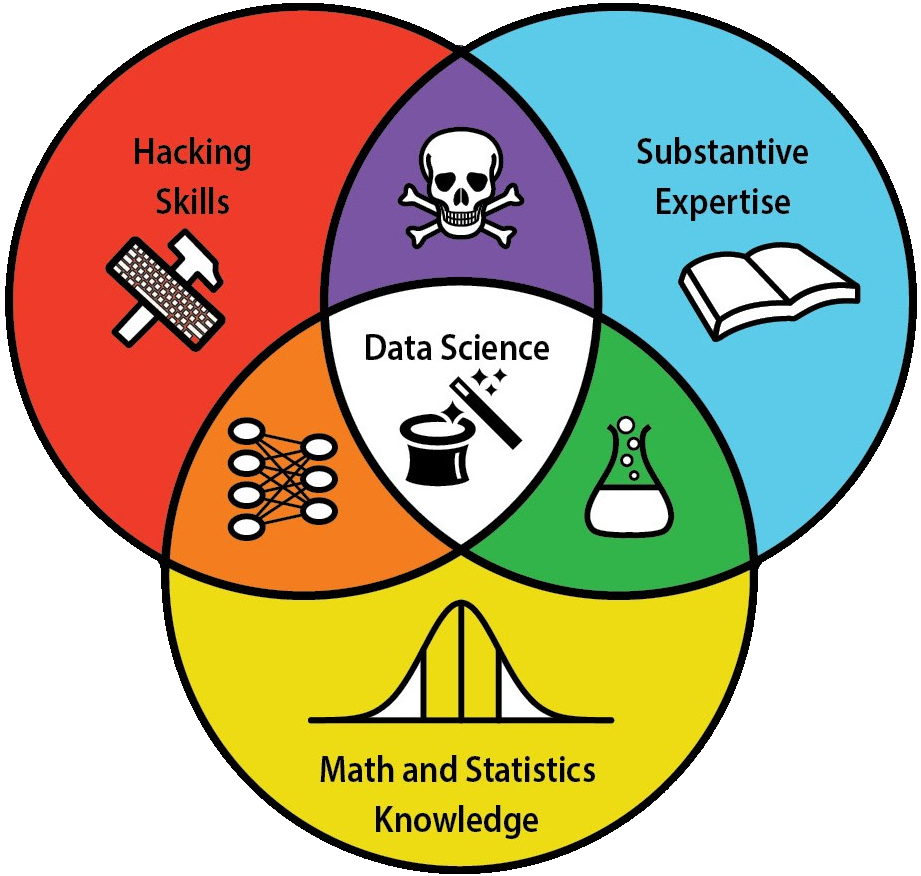
\includegraphics[width=7cm, height=7cm, keepaspectratio]{images/regresszio_1.png}
\end{center}
\end{column}
\end{columns}
\end{frame}

\begin{frame}{A gépi tanulás mögötti megfontolás}
A hagyományos szemléletmódban a programozó utasításokat írt egymás után a probléma megoldására.\par\smallskip
A gépi tanulás szemléletmódjában az algoritmus explicit programozás nélkül tanulja meg megoldani a problémát azáltal, hogy tapasztalat alapján tanul.
\begin{center}
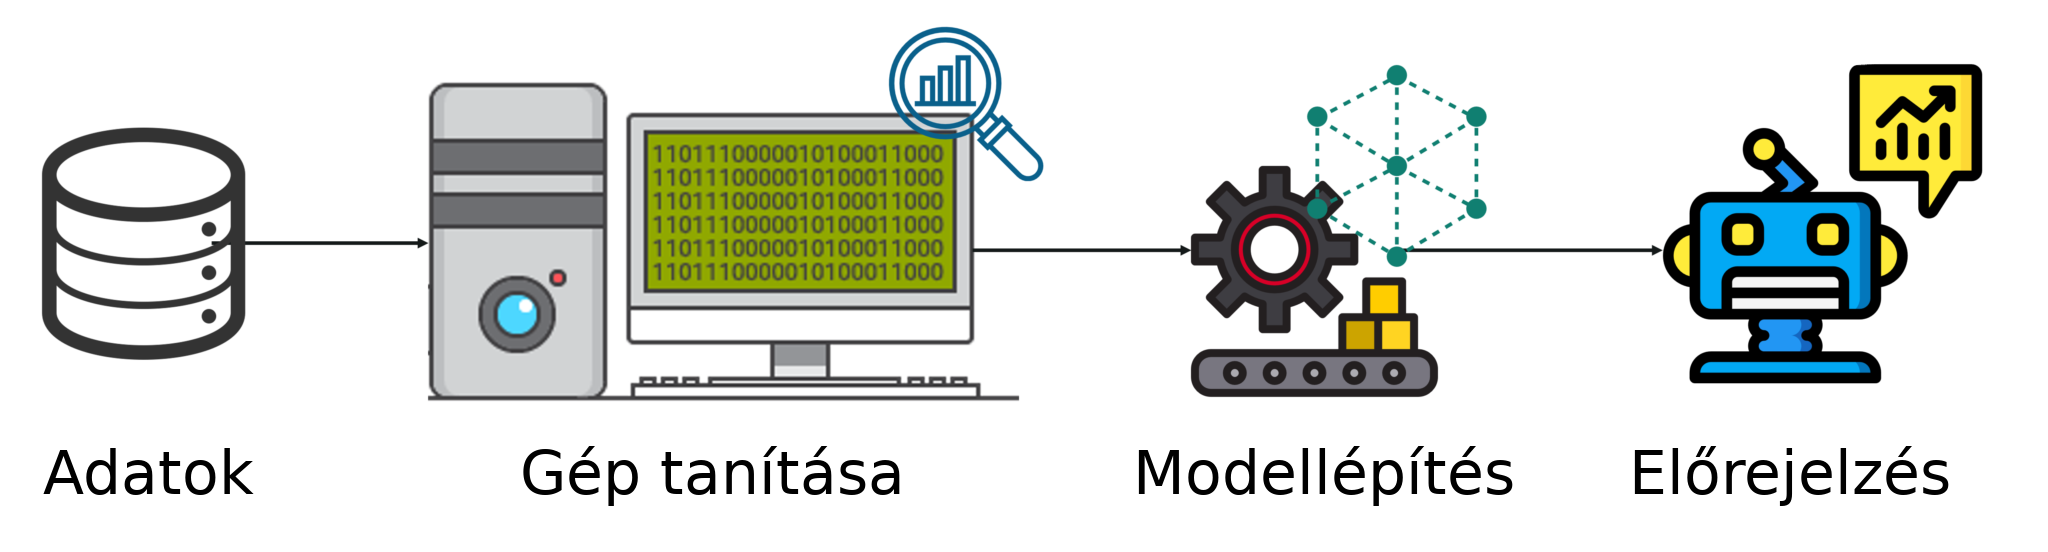
\includegraphics[width=12cm, height=7cm, keepaspectratio]{images/regresszio_2.png}
\end{center}
\end{frame}

\begin{frame}{A CRISP-DM módszertan}
\begin{columns}
\begin{column}{.5\textwidth}
A \textbf{C}ross \textbf{I}ndustry \textbf{S}tandard \textbf{P}rocess for \textbf{D}ata \textbf{M}ining egy folyamatmodell ami az
adatbányászati projektek folyamatát adja meg.
\begin{itemize}
	\item \textbf{Business understanding}: Üzleti igények felmérése
	\item \textbf{Data understanding}: Rendelkezésre álló adatok gyűjtése
	\item \textbf{Modeling}: Modell adatokra illesztése
	\item \textbf{Evaluation}: Illesztett modell kiértékelése
	\item \textbf{Deployment}: Átadás a tulajdonosoknak és használatba vétel
\end{itemize}
\end{column}
\begin{column}{.5\textwidth}
\begin{center}
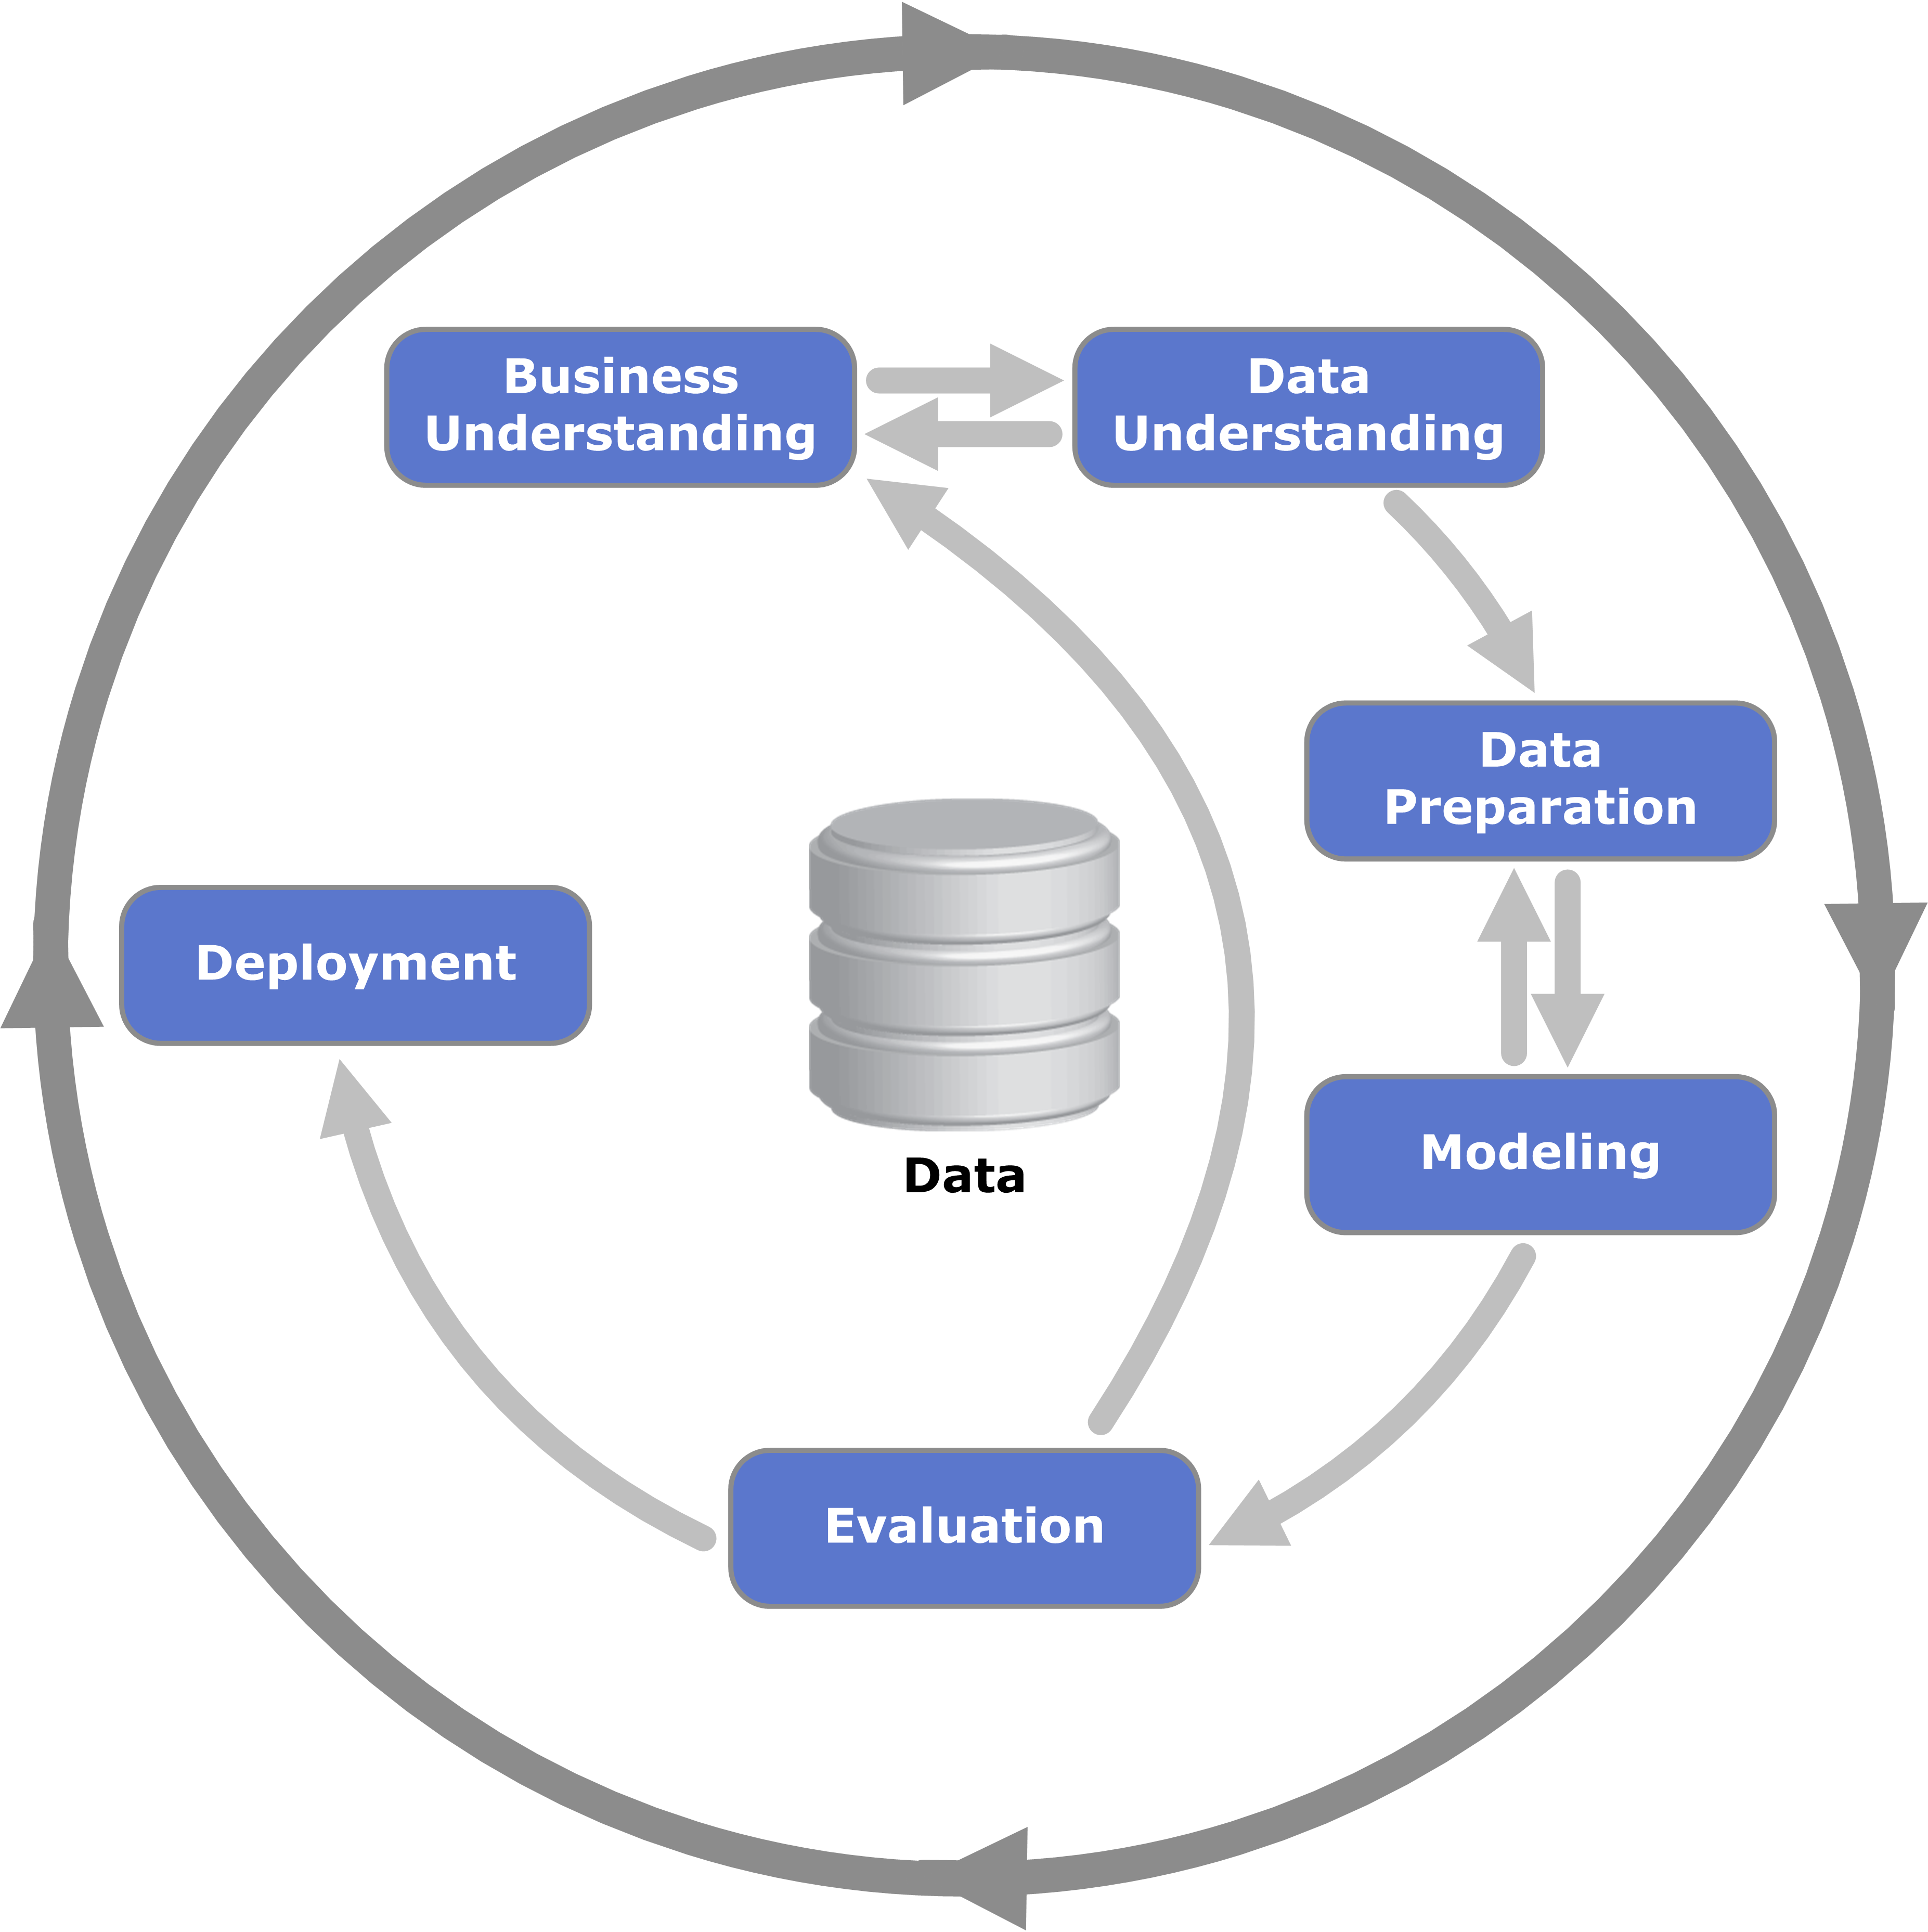
\includegraphics[width=7cm, height=7cm, keepaspectratio]{images/regresszio_3.png}
\end{center}
\end{column}
\end{columns}
\end{frame}

\begin{frame}{Kihívások a gépi tanulás területén}
\begin{columns}
\begin{column}{.5\textwidth}
\begin{itemize}
	\item Gyenge minőségű adatok
	\item Nem reprezentatív adatok
	\item Felesleges jellemzők
	\item Gép és ember kapcsolata
	\item Folyamatosan változó világ
	\item A problémák eredhetnek:
	\begin{itemize}
		\item Rossz változókból
		\item Rosszul általánosító algoritmusból
		\item Nehezen értelmezhető eredményekből
		\item Nagyon specifikus szakterületi specializációból
		\item Elégtelen minőségű vagy mennyiségű adatból
	\end{itemize}
\end{itemize}
\end{column}
\begin{column}{.5\textwidth}
\begin{center}
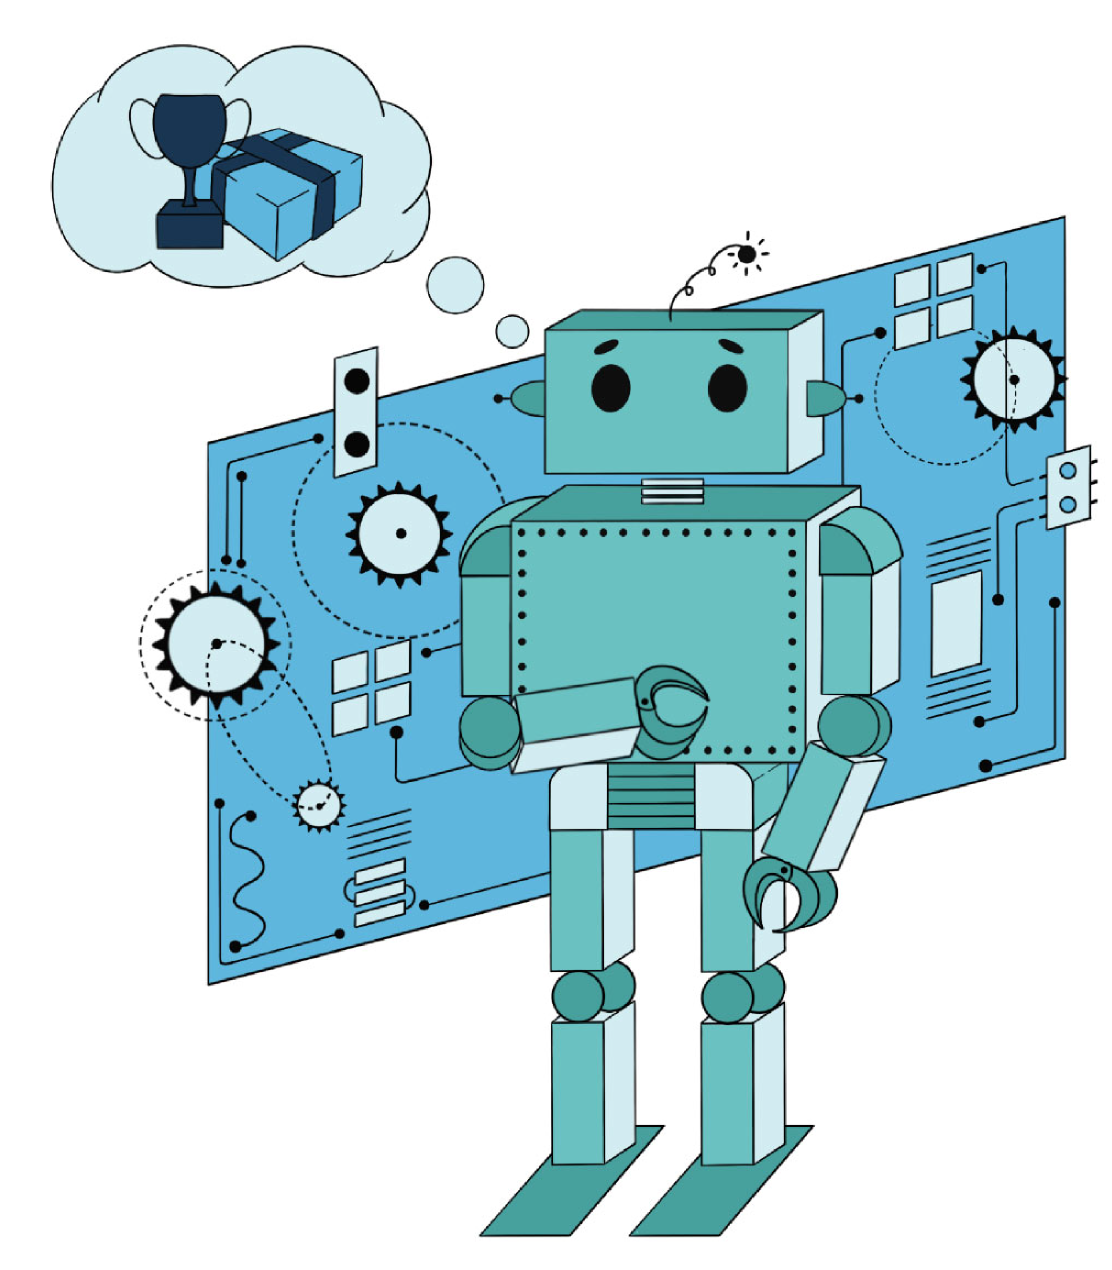
\includegraphics[width=7cm, height=7cm, keepaspectratio]{images/regresszio_9.png}
\end{center}
\end{column}
\end{columns}
\end{frame}

\section{Regresszió}

\begin{frame}
\tableofcontents[currentsection]
\end{frame}

\begin{frame}{Alapfogalmak}
\begin{columns}
\begin{column}{.5\textwidth}
\begin{block}{Regresszió}
Statisztikai elemző eljárás, amely változók közötti kapcsolatot modellez. Eredménye a \textbf{modell}.\par\smallskip
A regressziós elemzés \textbf{tárgya egy folytonos változó}.\par\smallskip
A \textbf{felügyelt tanulás} kategóriájába tartozik, tehát a modellezés során ismertek a kívánt outputok. 
\end{block}
\end{column}
\begin{column}{.5\textwidth}
\begin{center}
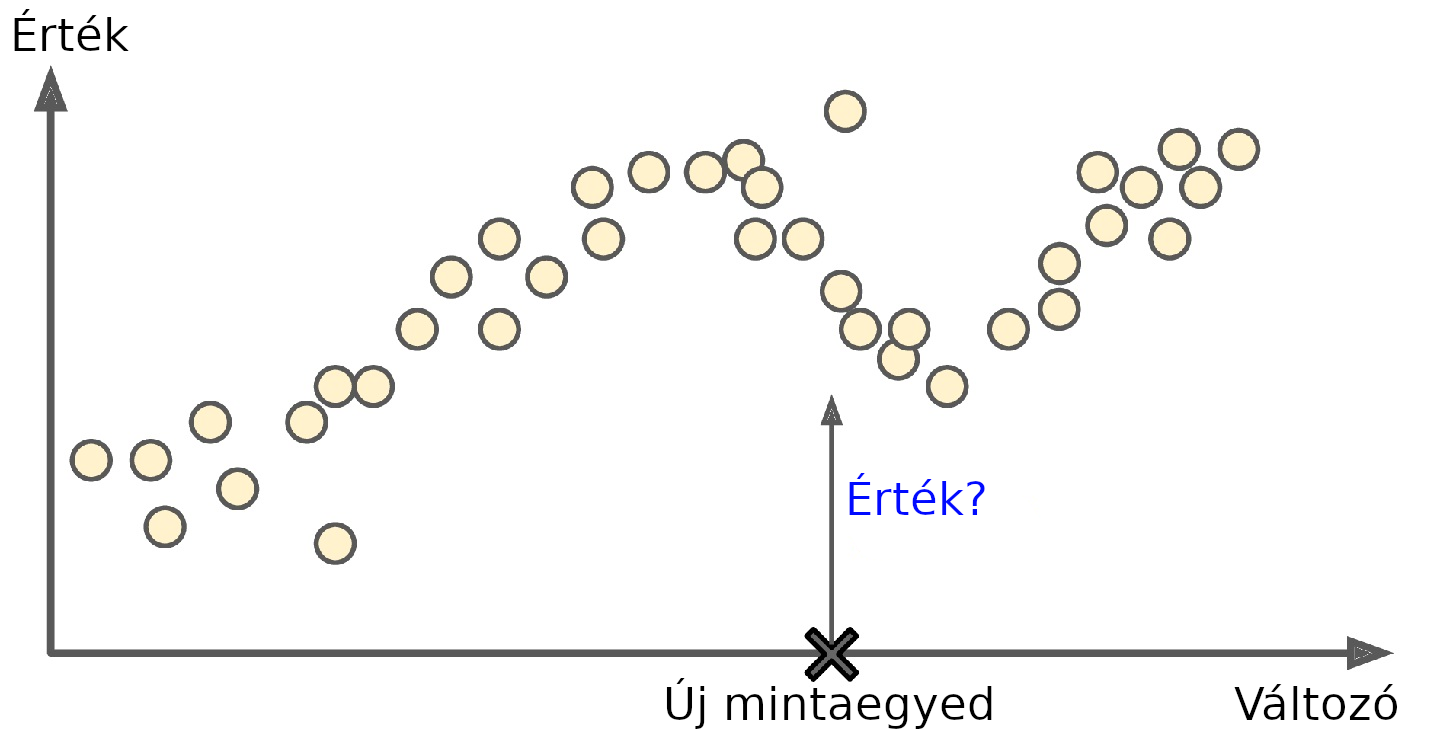
\includegraphics[width=7cm, height=7cm, keepaspectratio]{images/regresszio_8.png}
\end{center}
\end{column}
\end{columns}
\end{frame}

\begin{frame}{A regresszió komponensei}
\begin{columns}
\begin{column}{.5\textwidth}
\begin{itemize}
	\item \textbf{Célváltozó}: Egy jelenség, amely az elemzés tárgyát képezi. Példában: élet elégedettség. 
	\item \textbf{Független változó}: Azok a megfigyelések, amelyek alapján a célváltozó megbecsülhető. 
	\item \textbf{Modell}: A változók közötti feltételezett kapcsolat, ami a valóságot leírja.
\end{itemize}
\end{column}
\begin{column}{.5\textwidth}
\begin{center}
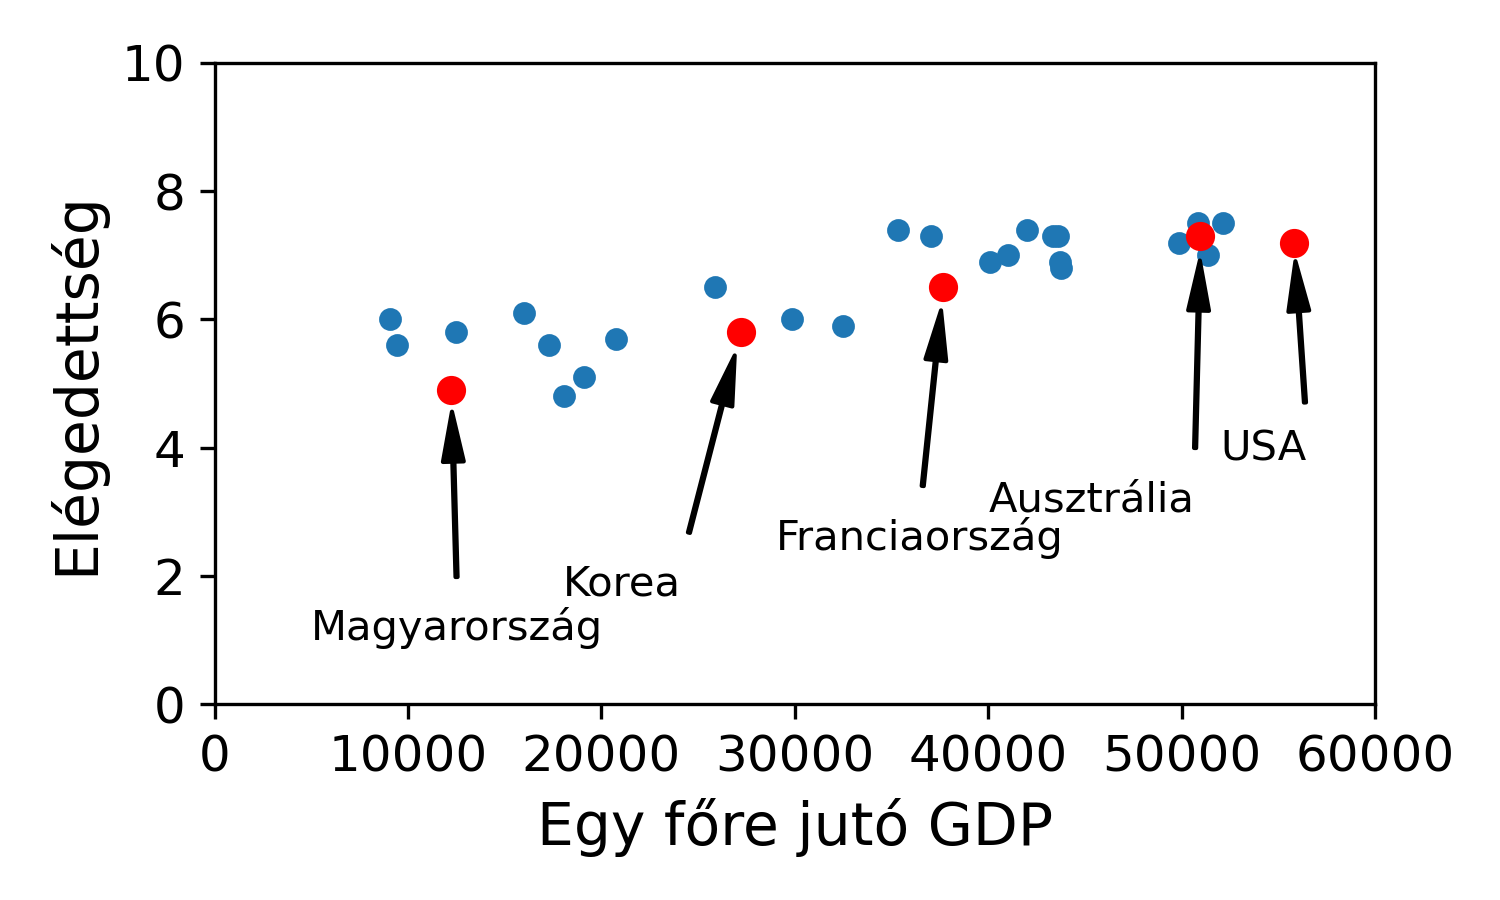
\includegraphics[width=7cm, height=7cm, keepaspectratio]{images/regresszio_4.png}
\end{center}
\end{column}
\end{columns}
\end{frame}

\begin{frame}{A regresszió alkalmazása}
\begin{columns}
\begin{column}{.5\textwidth}
Tipikusan akkor használatosak a regressziós eljárások, amikor a vizsgálat tárgya, hogy \textbf{egyes jelenségek hogyan befolyásolnak másokat}. Ezzel lehetséges annak a feltárása, hogy milyen \textbf{kapcsolati rendszer szerint hozhatók összefüggésbe}.\par\smallskip
Regresszió segítségével lehetséges \textbf{valamilyen választ előre jelezni}.\par\smallskip
Például meg lehet jósolni az egy országban élők saját életükkel való elégedettséget az ország egy főre jutó GDP mutatója alapján. 
\end{column}
\begin{column}{.5\textwidth}
\only<1>{\begin{center}
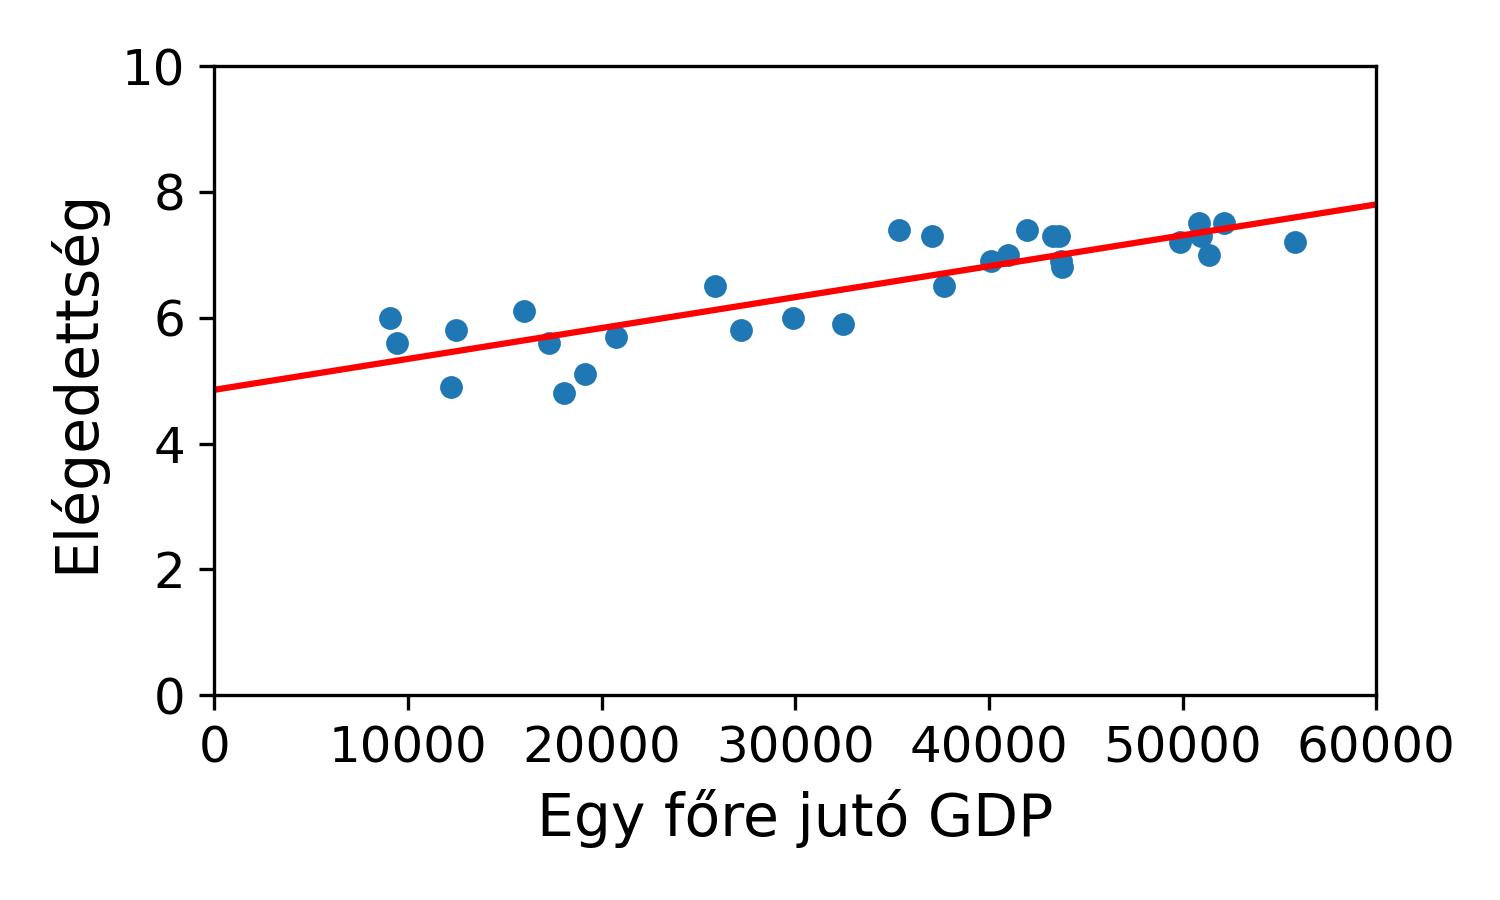
\includegraphics[width=7cm, height=7cm, keepaspectratio]{images/regresszio_5.png}
\end{center}}
\only<2>{\begin{center}
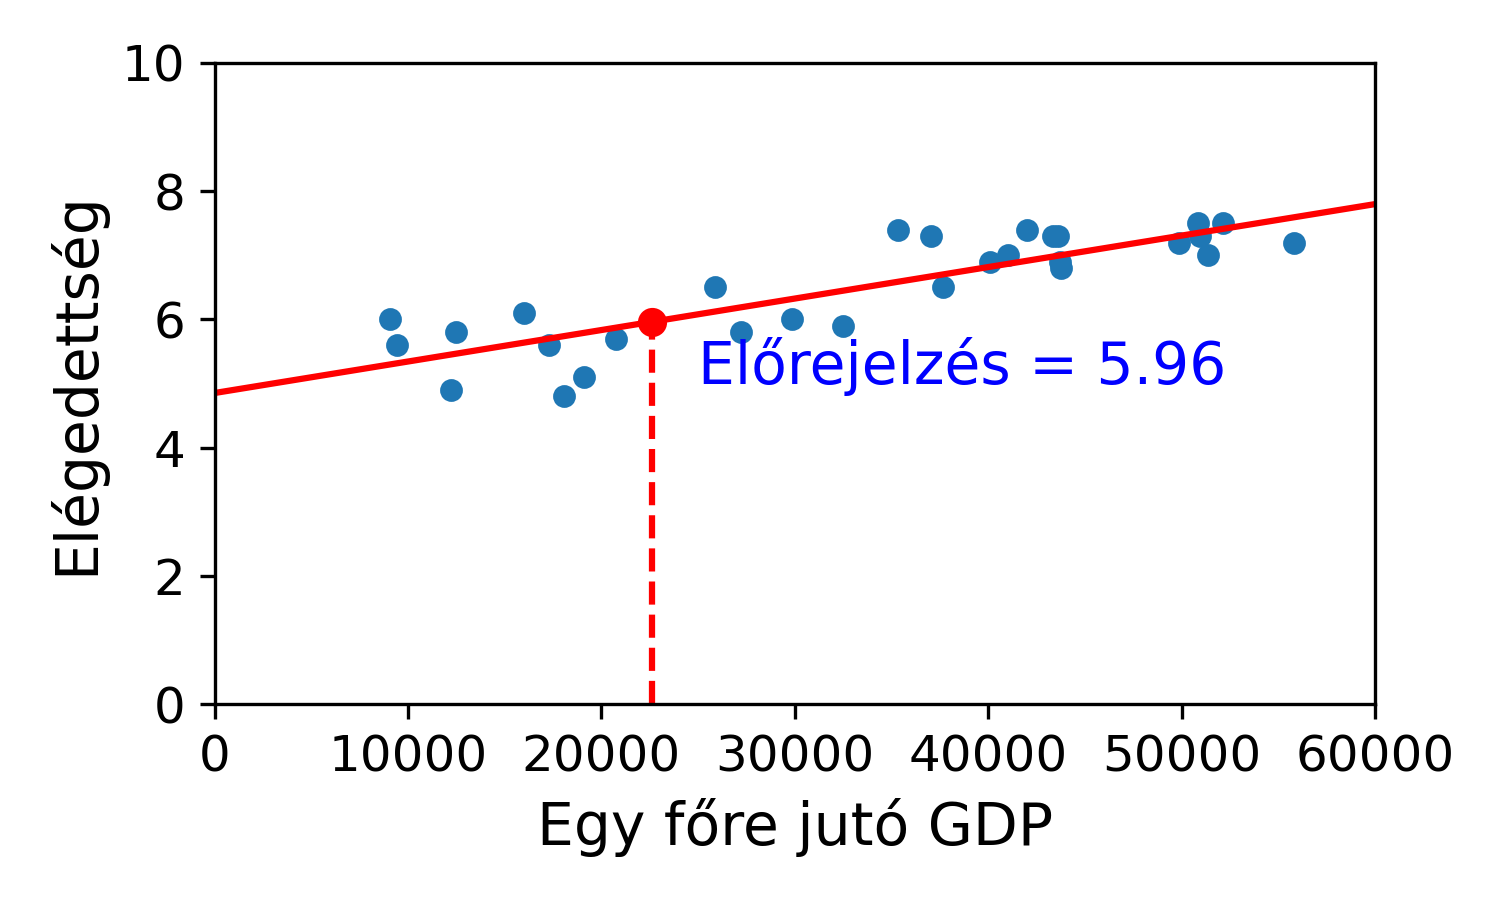
\includegraphics[width=7cm, height=7cm, keepaspectratio]{images/regresszio_6.png}
\end{center}}
\end{column}
\end{columns}
\end{frame}

\begin{frame}{A regresszió felírása}
\begin{columns}
\begin{column}{.5\textwidth}
A lineáris regresszió célja, hogy valamely $y$ változót megbecsülje adott $x=\left(x_1,x_2,\ldots,x_r \right)$ magyarázó változók alapján.
\begin{block}{Lineáris regresszió}
A regresszió egyenlete:
\[
\hat{y} = \theta_0 + \theta_1 \cdot x + \varepsilon
\]
Ahol $\hat{y}$ a becsült érték, $\theta$ értékek a regressziós együtthatók vagy \textbf{paraméterek}, $\varepsilon$ pedig a véletlen hiba.
\end{block}
Ebben az esetben $\theta_0$ az egyenes eltolása, $\theta_1$ pedig a meredeksége. 
\end{column}
\begin{column}{.5\textwidth}
\begin{center}
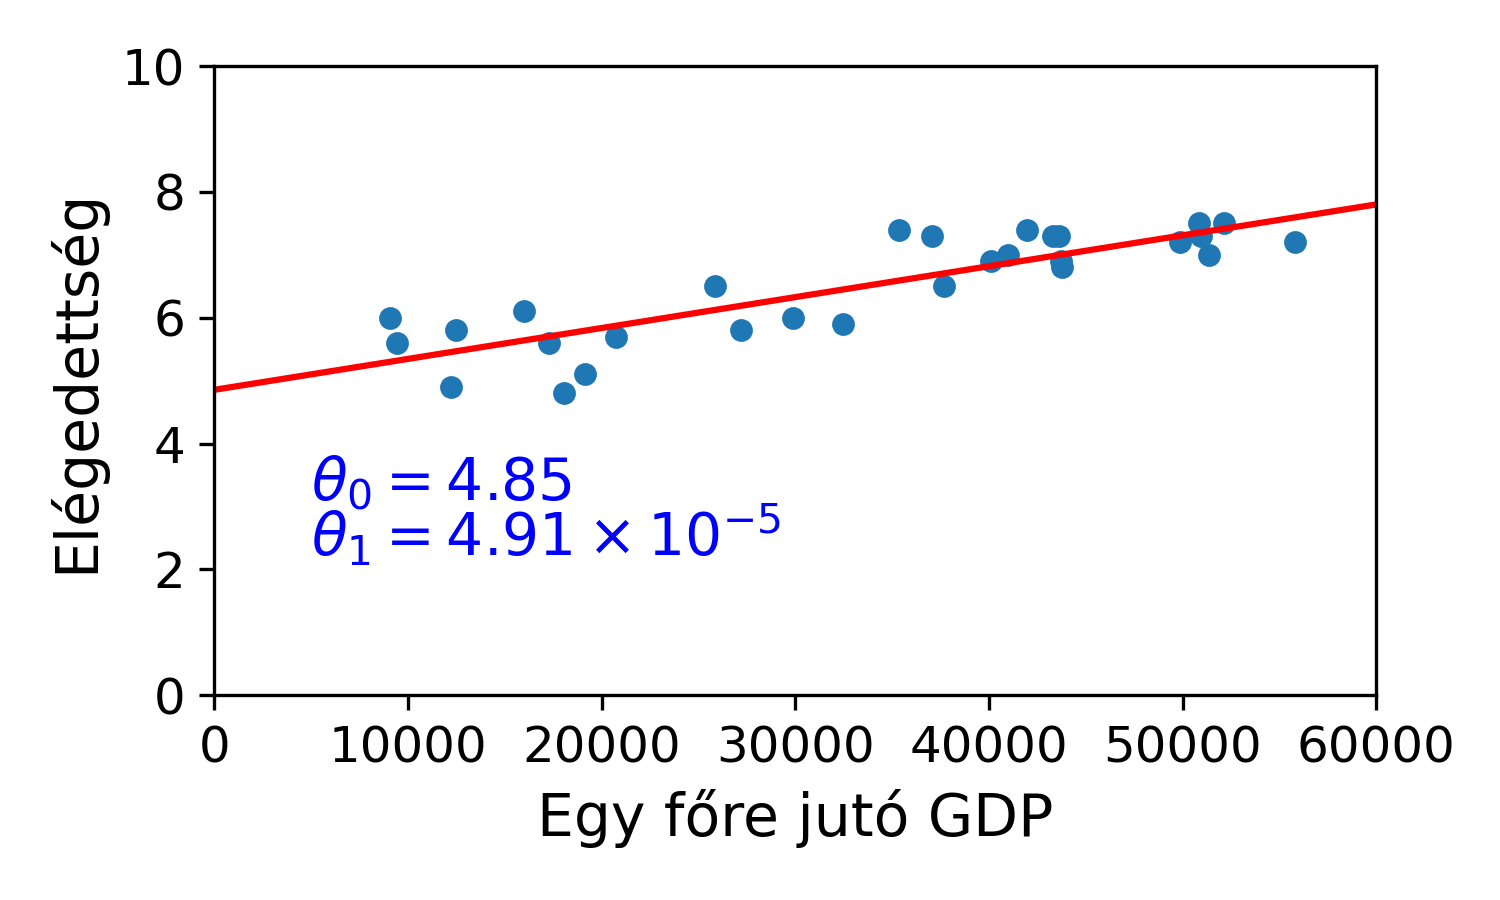
\includegraphics[width=7cm, height=7cm, keepaspectratio]{images/regresszio_7.png}
\end{center}
\end{column}
\end{columns}
\end{frame}

\begin{frame}{A regresszió teljesítménye}
\begin{columns}
\begin{column}{.5\textwidth}
A gépi tanulás esetén szükség van arra, hogy meglehessen mondani, mennyire jó a modell. Regresszió esetén a feladat a legkisebb hibához tartozó modell megkeresése.
\begin{center}
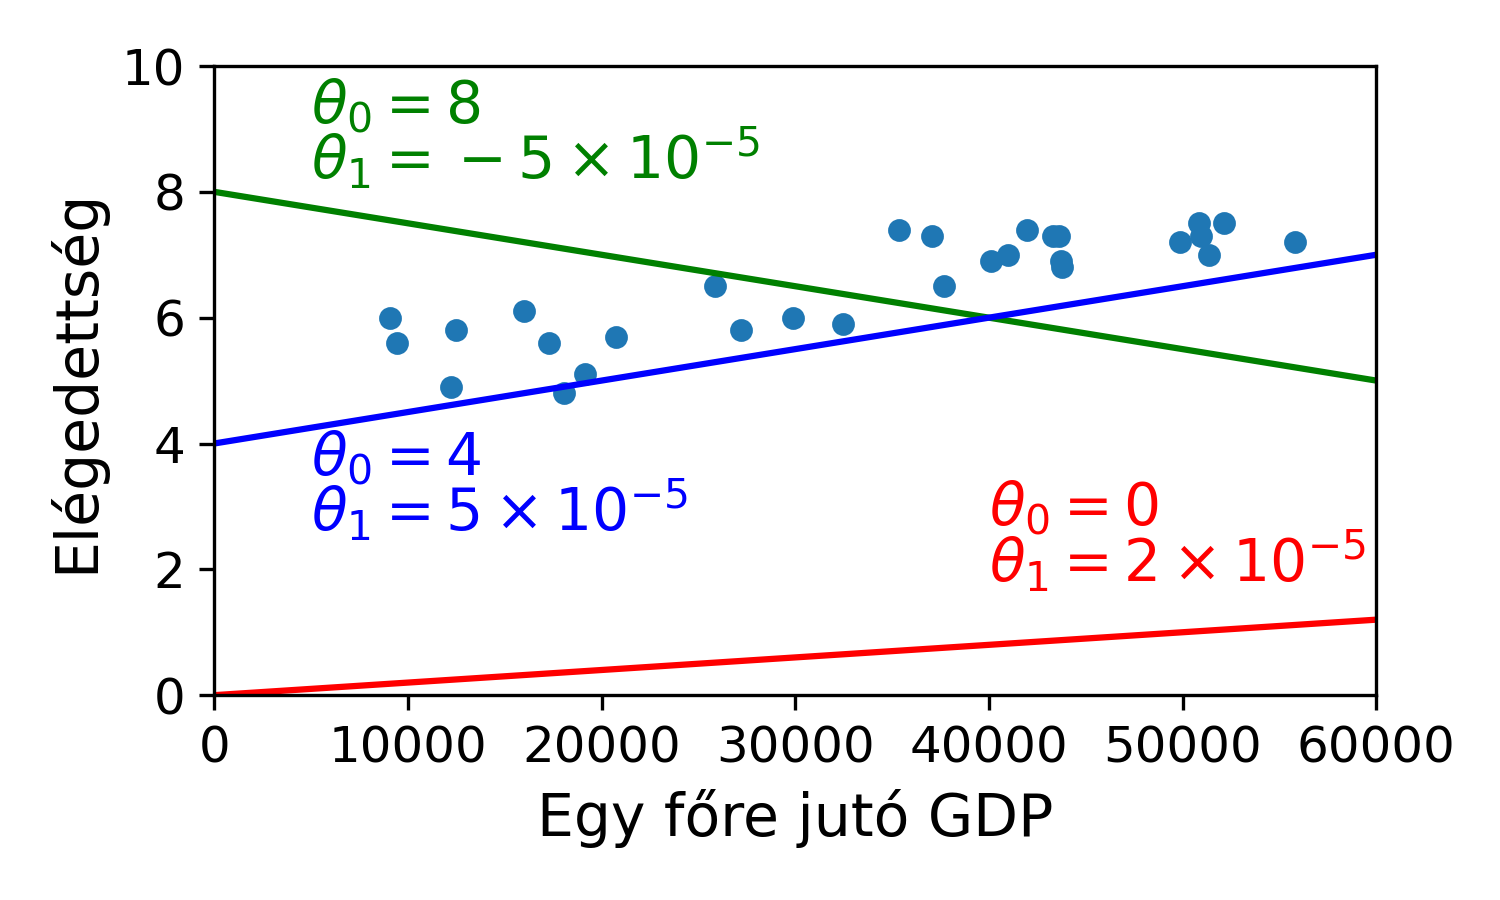
\includegraphics[width=7cm, height=7cm, keepaspectratio]{images/regresszio_11.png}
\end{center}
\end{column}
\begin{column}{.5\textwidth}
\begin{block}{Rezidum}
Az $y_i$ valós érték és $\hat{y}_i$ becsült érték távolsága adott $d$ távolságfüggvény szerint:
\[
r_i = d\left( y_i,\hat{y}_i \right), \; r_i \in \mathbb{R}
\]
\end{block}
\begin{block}{Költségfüggvény}
A rezidumok összege az összes minta adatpontra:
\[
L\left( y,\hat{y}  \right) = \sum_{i=1}^n r_i = \sum_{i=1}^n d\left( y_i,\hat{y}_i \right)
\]
\end{block}
\end{column}
\end{columns}
\end{frame}

\begin{frame}{Hiba kiszámítása MSE módszerrel}
\begin{columns}
\begin{column}{.5\textwidth}
Az egyik legismertebb költségfüggvény az átlagos négyzetes hiba.
\begin{block}{MSE (Mean Squared Error)}
\[
MSE = \frac{1}{n} \sum_{i=1}^n \left( y_i - \hat{y}_i \right)^2
\]
Ahol $y_i$ az aktuális minta adatpont és $\hat{y}_i$ a regressziós modell által adott becsült érték. 
\end{block}
\end{column}
\begin{column}{.5\textwidth}
\begin{center}
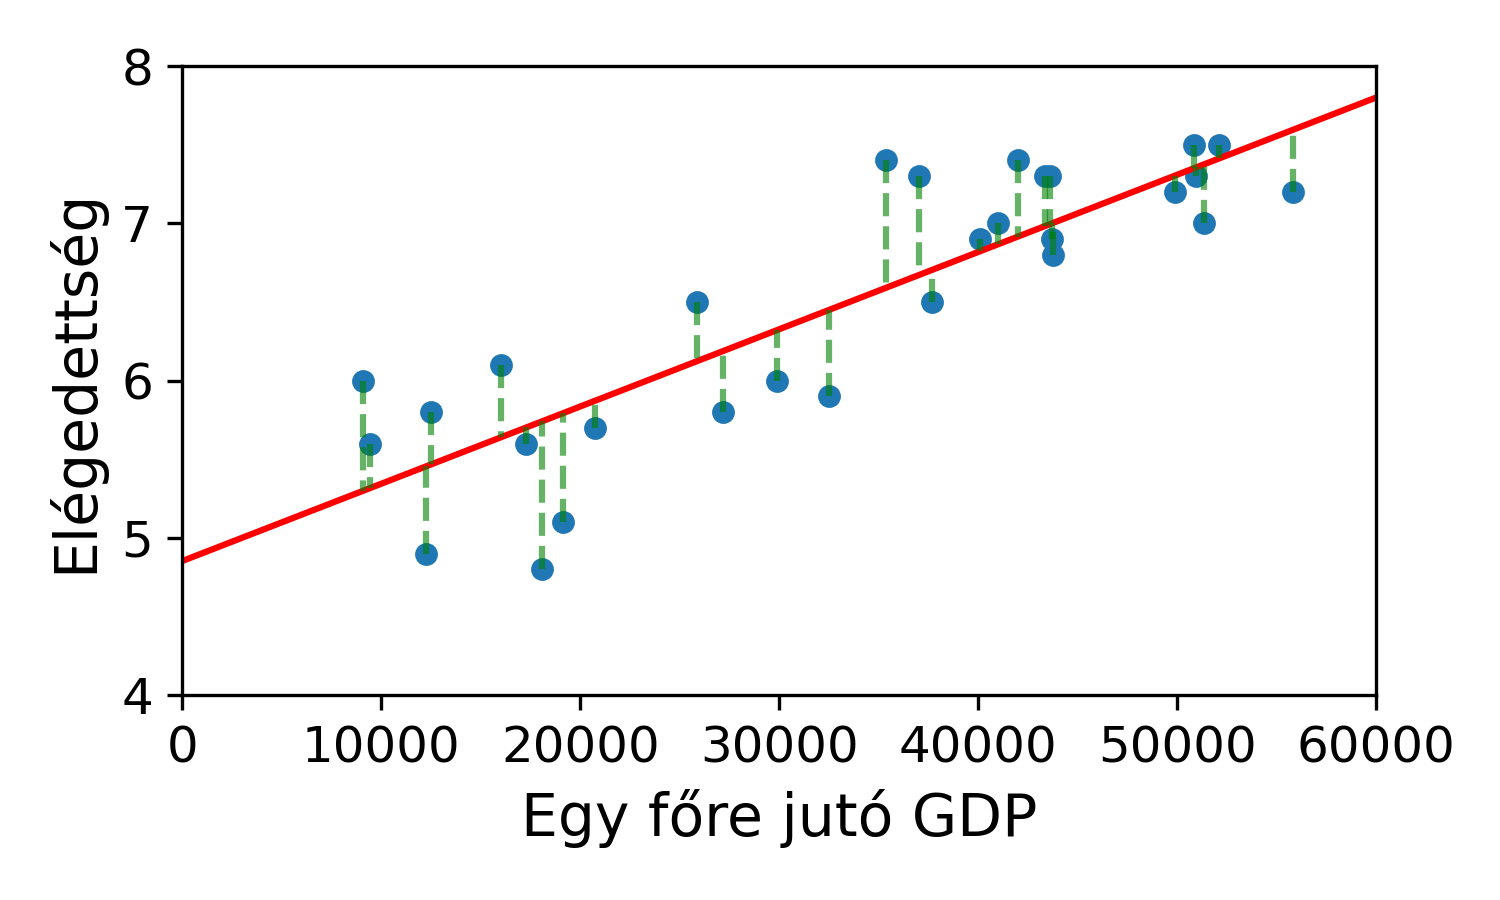
\includegraphics[width=7cm, height=7cm, keepaspectratio]{images/regresszio_10.png}
\end{center}
\end{column}
\end{columns}
\end{frame}

\section{Optimalizáció}

\begin{frame}
\tableofcontents[currentsection]
\end{frame}

\begin{frame}{Alultanulás és túltanulás}
\begin{columns}
\begin{column}{.5\textwidth}
A gépi tanulásban két egymással ellentétes célra kell optimalizálni a modelleket. Ez a jó általánosító képesség és a pontos becslés. 
\only<1>{\begin{block}{Alultanulás}
Alultanulás esetén az illesztett modell \textbf{túlságosan általános}, nem képes hitelesen leképezni a valóságban rejlő komplex kapcsolati rendszert. Az alultanult modell \textbf{egyformán rosszul teljesít mind a tanító és előre nem látott adatokon}.
\end{block}}
\only<2>{\begin{block}{Túltanulás}
Túltanulás esetén a modell nagyon pontosan, akár hiba nélkül illeszkedik a tanító adatpontokra, de \textbf{komplexitása miatt elveszíti a jó általánosító képességét}, és nem fog jól teljesíteni előre nem látott adatokon.
\end{block}}
\only<3>{\begin{block}{Optimális modell}
Az optimális modell \textbf{egyszerre} képezi le hűen a valóság kapcsolatait és általánosít olyan módon, hogy az előre nem látott adatokon is jó előrejelzéseket legyen képes adni. 
\end{block}}
\end{column}
\begin{column}{.5\textwidth}
\only<1>{\begin{center}
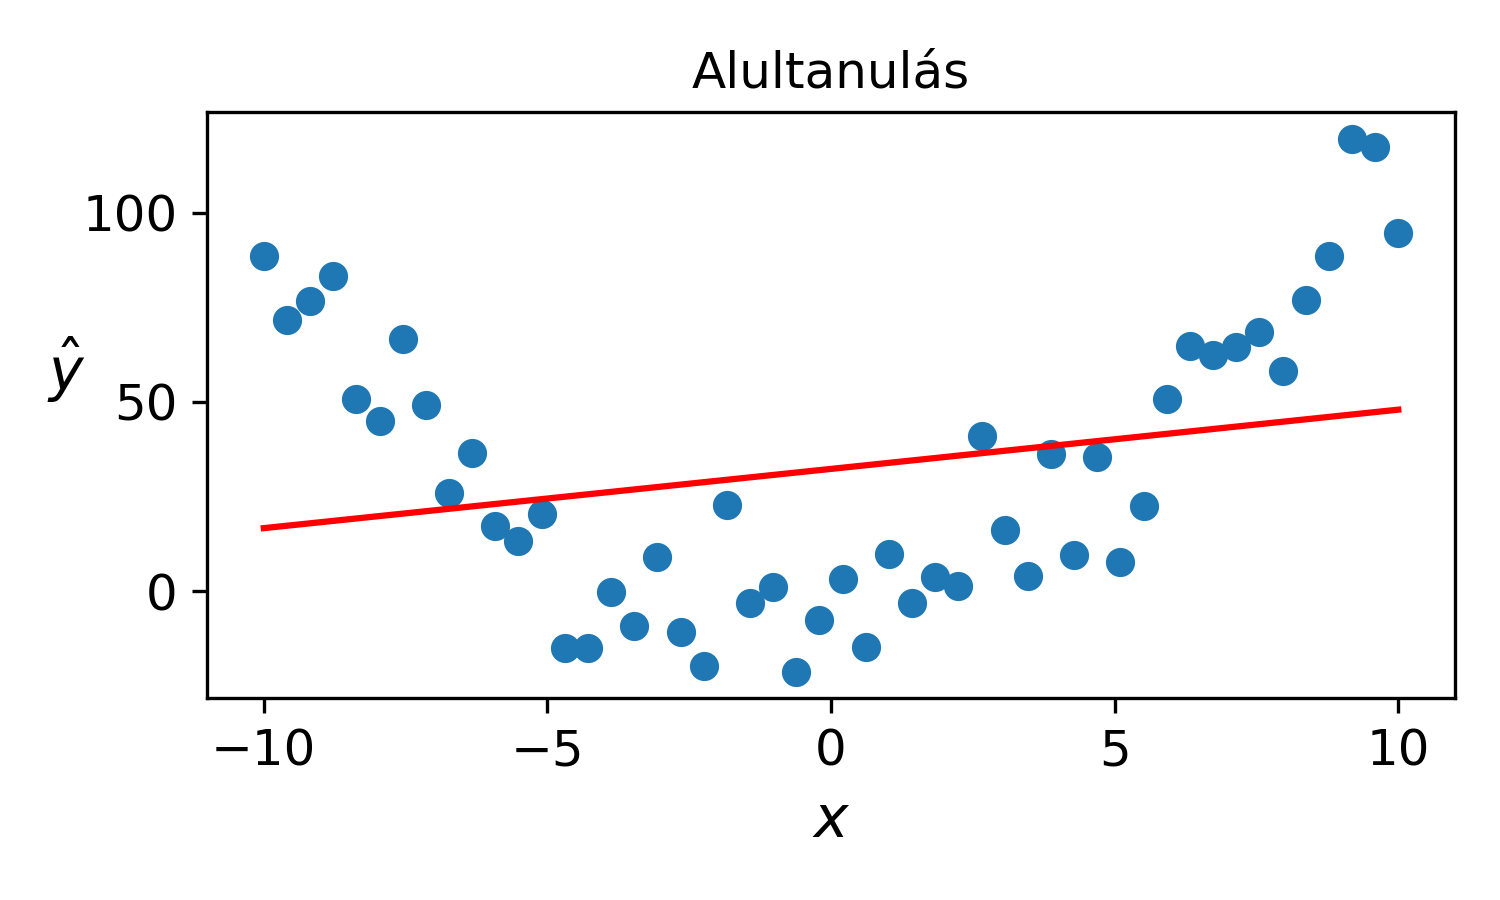
\includegraphics[width=7cm, height=7cm, keepaspectratio]{images/regresszio_12.png}
\end{center}}
\only<2>{\begin{center}
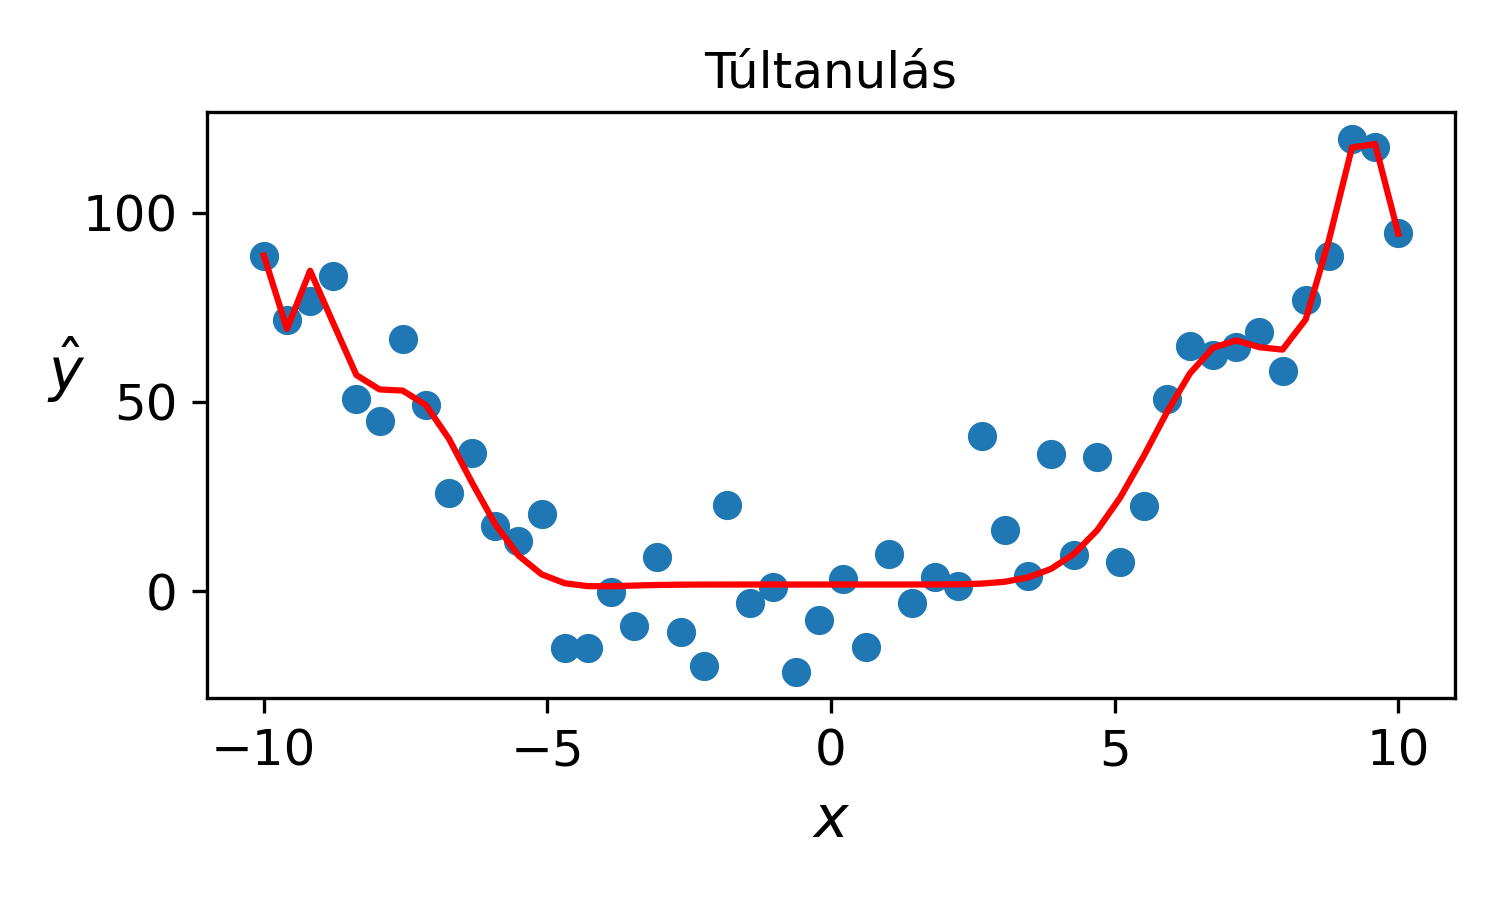
\includegraphics[width=7cm, height=7cm, keepaspectratio]{images/regresszio_13.png}
\end{center}}
\only<3>{\begin{center}
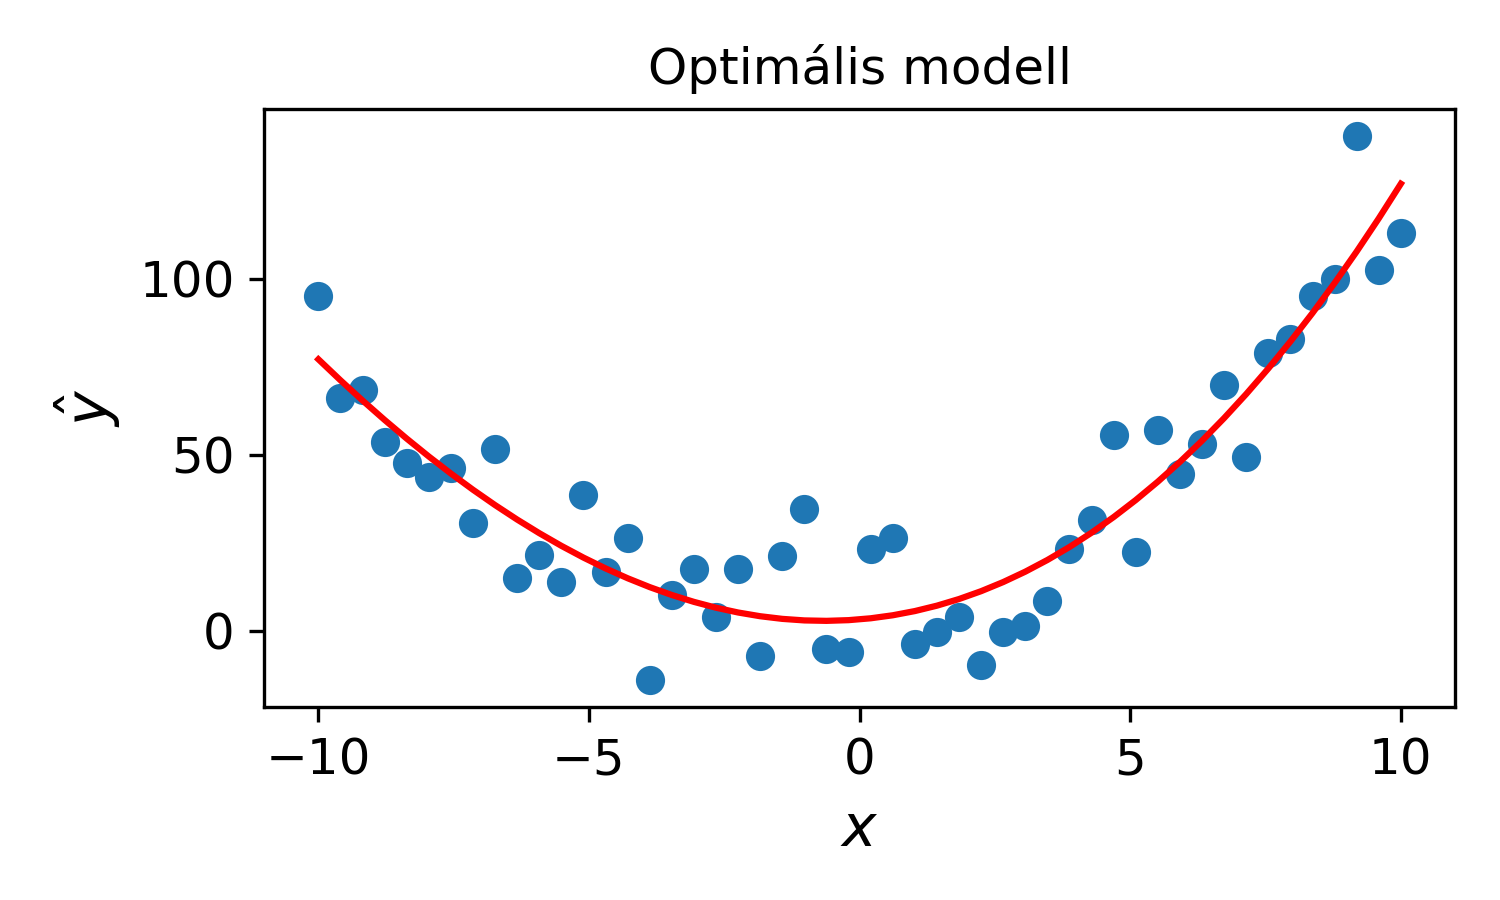
\includegraphics[width=7cm, height=7cm, keepaspectratio]{images/regresszio_14.png}
\end{center}}
\end{column}
\end{columns}
\end{frame}

\begin{frame}{Torzítás és variancia}
\begin{columns}
\begin{column}{.5\textwidth}
A modellezés két szélsőértéke a torzítás és variancia.
\only<1>{\begin{block}{Torzítás}
Ez arra utal, hogy \textbf{mennyire jól képes a modell leképezni a valós kapcsolatokat} a tanító adatokon.
\end{block}
Magas torzítás azt jelenti, hogy a modell túlságosan egyszerű, és nem képes megragadni az adatok összefüggéseit.}
\only<2>{\begin{block}{Variancia}
A variancia azt mutatja meg, hogy a modell \textbf{hogyan reagál a különböző tanító adatkészletekre}.
\end{block}
Magas variancia esetén a modell túlzottan érzékeny a tanító adatok kis változásaira, tehát túlilleszti magát a tanító adatokra, és nem képes jól generalizálni új, látatlan adatokra.}
\end{column}
\begin{column}{.5\textwidth}
\begin{center}
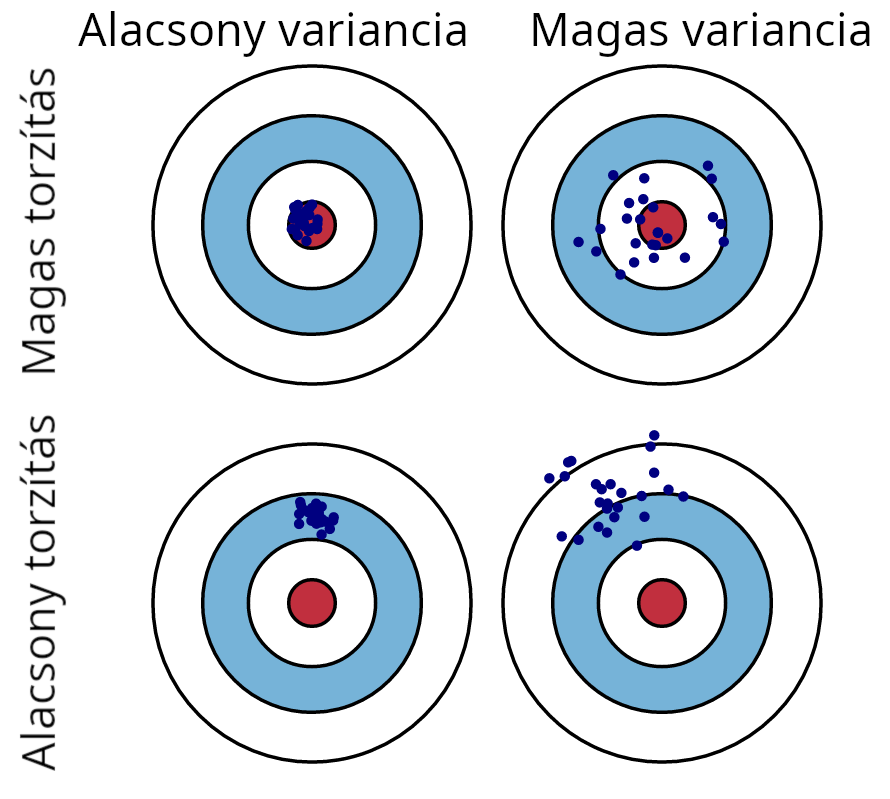
\includegraphics[width=7cm, height=7cm, keepaspectratio]{images/regresszio_15.png}
\end{center}
\end{column}
\end{columns}
\end{frame}

\begin{frame}{A modell optimalitása}
\begin{columns}
\begin{column}{.5\textwidth}
A modellezés során egyszerre kell úgy illeszteni a függvényt, hogy jól általánosítson, ugyanakkor a valóság kapcsolatait ne hamisítsa meg.\par\medskip
Amikor a tanítás elején a modell nagyon egyszerű, jól képes általánosítani, viszont a hibája magas lesz a tanító adatpontokon.\par\medskip
Ahogy egyre tanultabb lesz a modell a hiba csökkenni fog, viszont annál specializáltabb lesz és veszíti el az általánosító képességét. 
\end{column}
\begin{column}{.5\textwidth}
\begin{center}
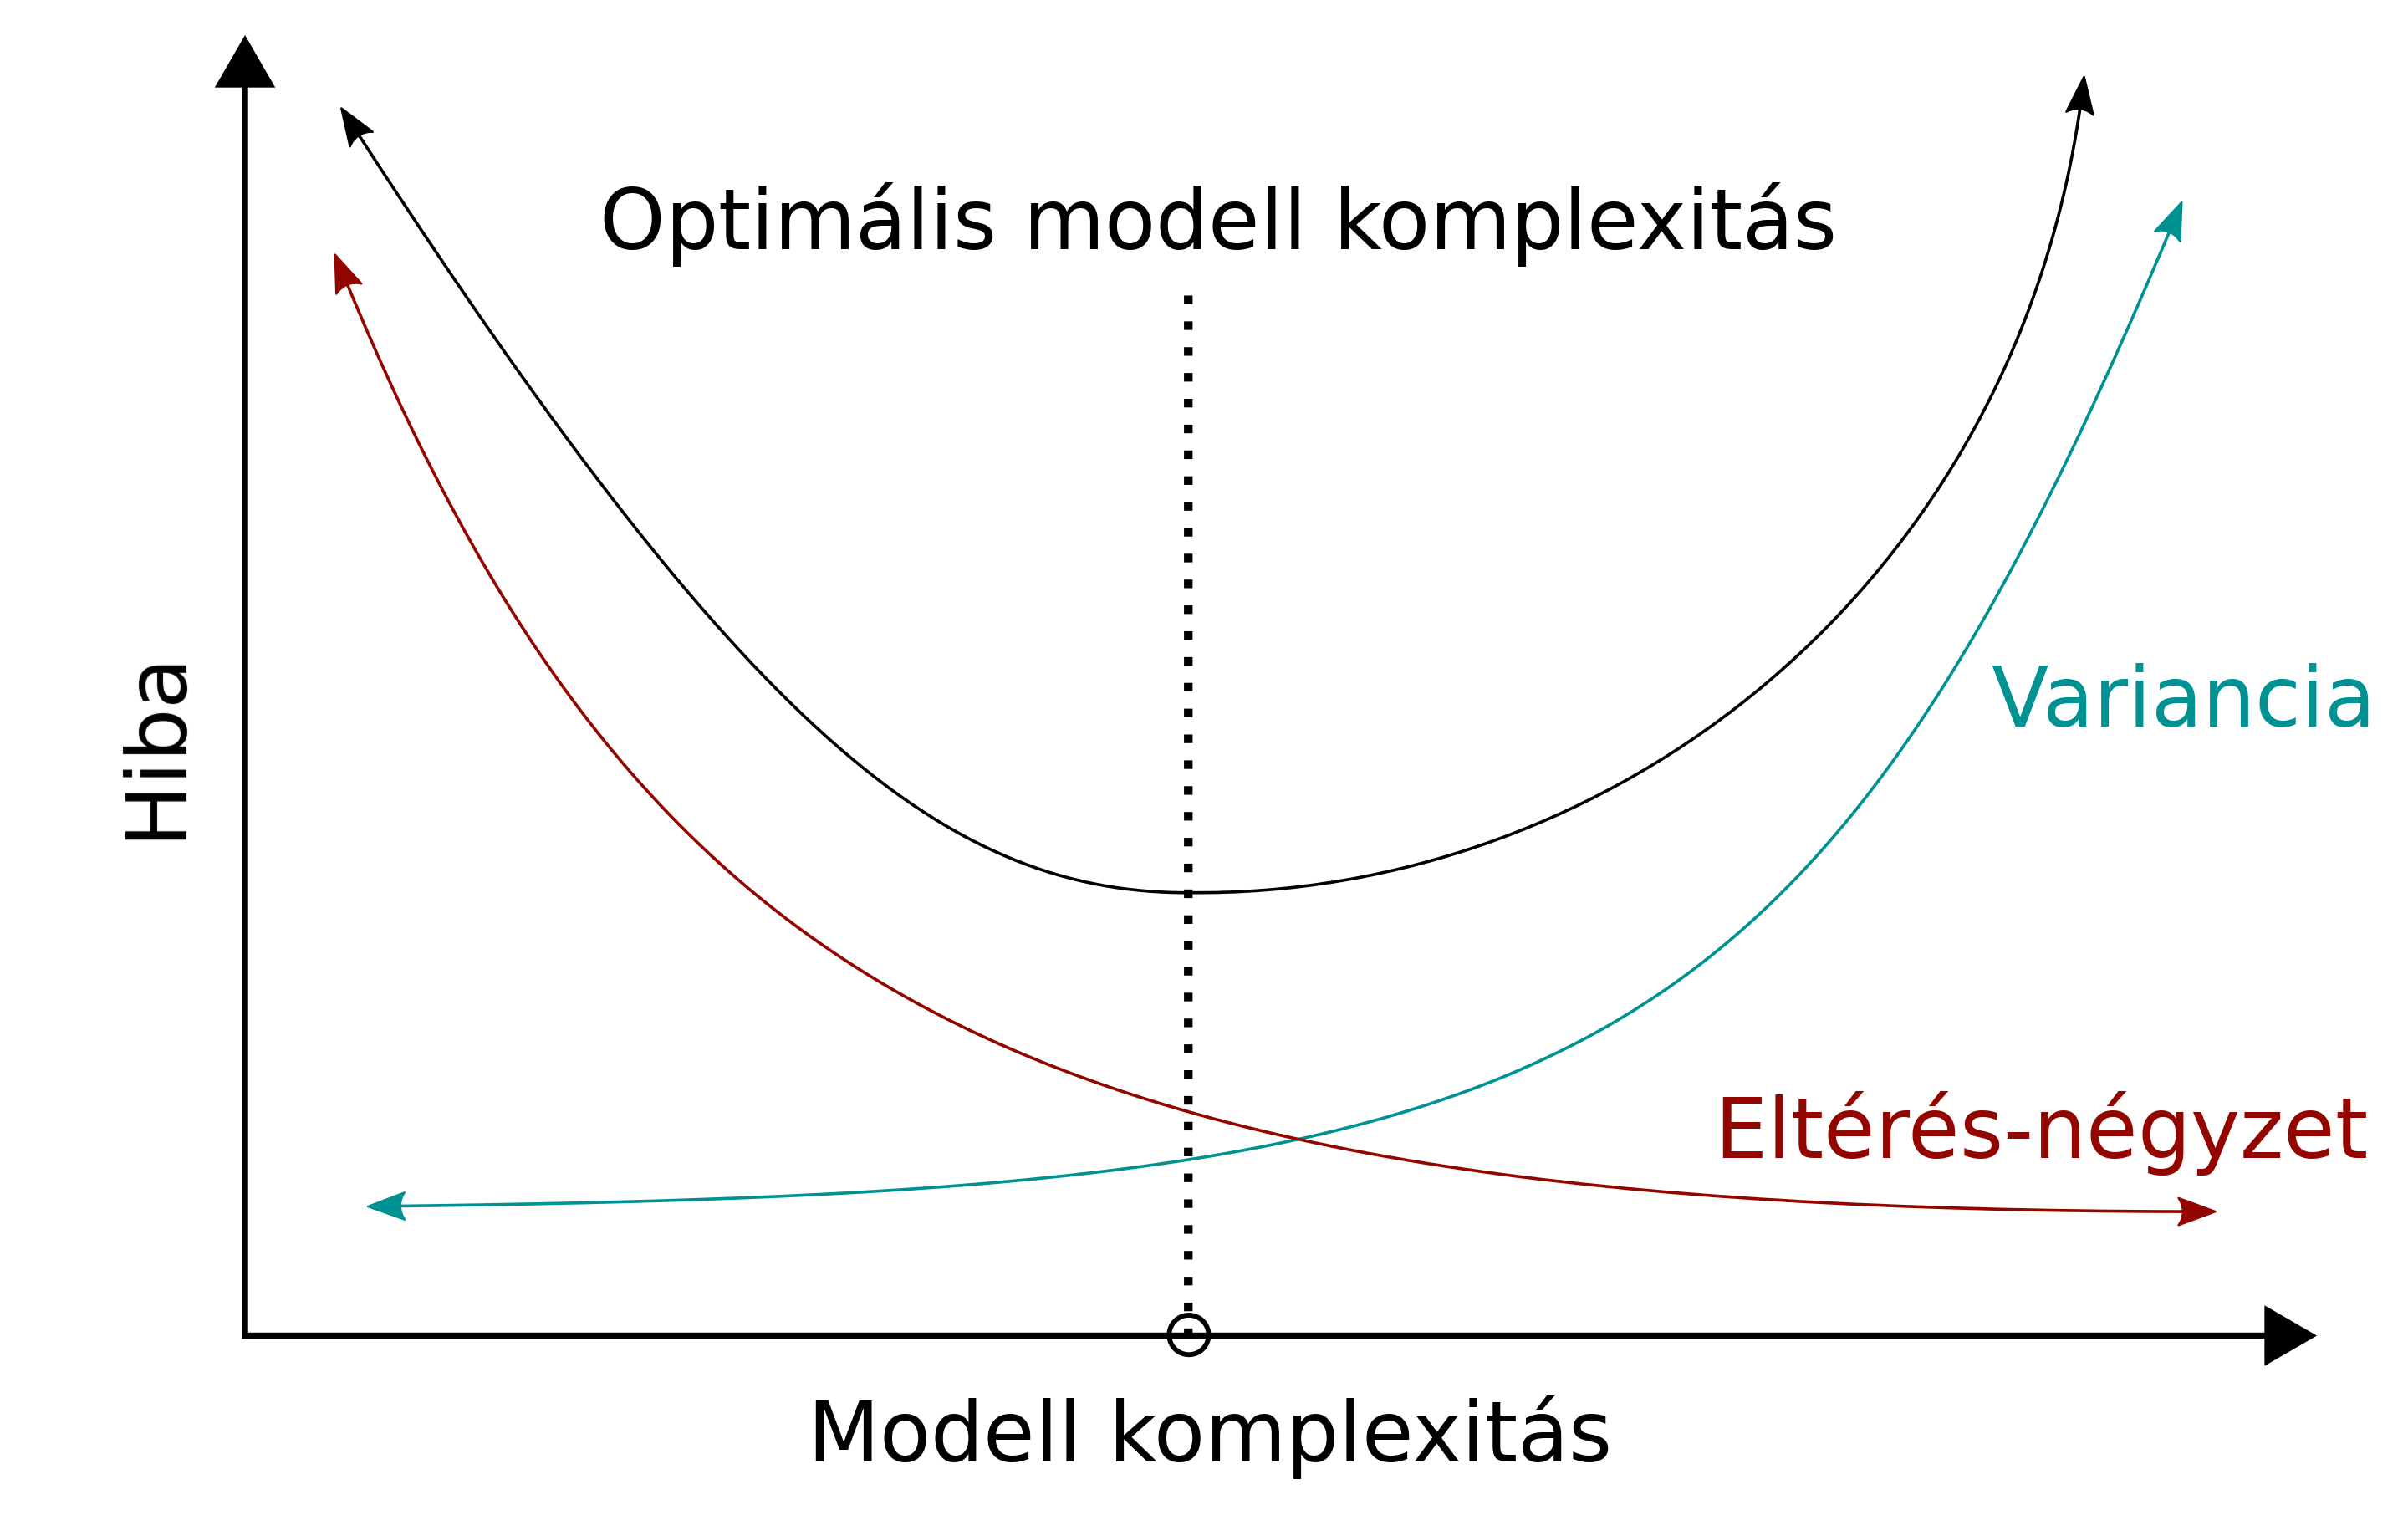
\includegraphics[width=7cm, height=7cm, keepaspectratio]{images/regresszio_16.png}
\end{center}
\end{column}
\end{columns}
\end{frame}

\section{Gradiens ereszkedés}

\begin{frame}
\tableofcontents[currentsection]
\end{frame}

\begin{frame}{Gradiens}
\begin{columns}
\begin{column}{.5\textwidth}
\begin{block}{Gradiens}
Egy $f\left( x,y,z \right)$ függvény esetén gradiens egy olyan vektor, amely arra az irányra mutat, ahol az $f$ függvény a legmeredekebben emelkedik.\par\smallskip
Ha $f$ 3D térben van definiálva, $\left( x,y,z \right)$ koordinátákkal, a gradiens: 
\[
\nabla f = \left[ \frac{\partial f}{\partial x}, \frac{\partial f}{\partial y}, \frac{\partial f}{\partial z} \right]
\]
A gradiens tetszőleges dimenziószámra általánosítható. 
\end{block}
\end{column}
\begin{column}{.5\textwidth}
\begin{center}
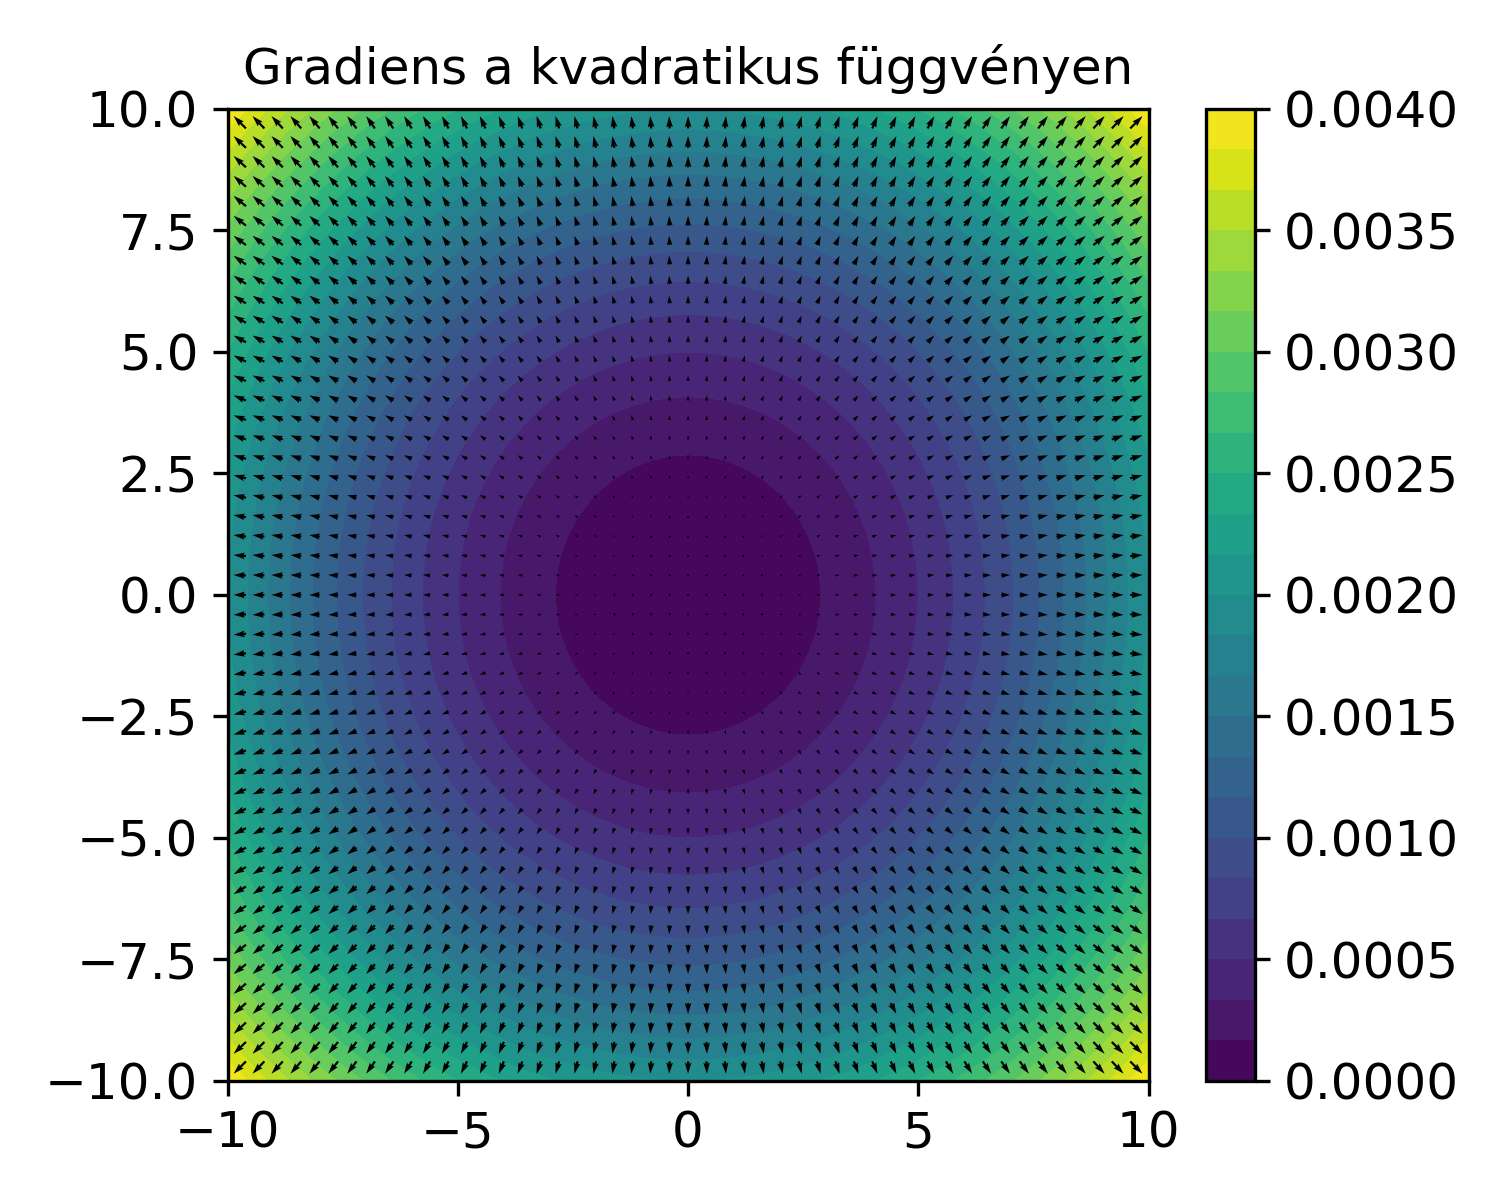
\includegraphics[width=7cm, height=7cm, keepaspectratio]{images/regresszio_17.png}
\end{center}
\end{column}
\end{columns}
\end{frame}

\begin{frame}{Gradiens ereszkedés}
\begin{columns}
\begin{column}{.5\textwidth}
\only<1>{\begin{block}{Gradiens ereszkedés}
Iteratív optimalizálási módszer \textbf{egy célfüggvény minimum helyének megtalálására}, amely a célfüggvény gradiensét használja a keresési irány meghatározására. 
\end{block}
Az eljárás alapvető elgondolása, hogy a függvény gradiensének ellentétes irányában haladva eljut a legkisebb értékhez, mivel a gradiens a függvény növekedésének legnagyobb irányát mutatja.}
\only<2>{Egy alapvető algoritmus gradiens ereszkedésre:
\begin{algorithm}[H]
\caption{Gradiens ereszkedés}
\SetAlgoLined
\textbf{Input}: $\alpha$, $f(\theta)$\\
$\theta_0 \leftarrow 0$\;
\For{$t = 0 \rightarrow max_t$}{
	$\nabla f(\theta_t)$ gradiens kiszámítása\;
	$\theta_{t+1} = \theta_t - \alpha \cdot \nabla f(\theta_t)$\;
}
\end{algorithm}
Ahol $\theta$ a célfüggvényt meghatározó paraméterek vektora, $\nabla f(\theta_t)$ a célfüggvény gradiense, $\alpha \in [0,1]$ a tanulási sebesség.
}
\end{column}
\begin{column}{.5\textwidth}
\begin{center}
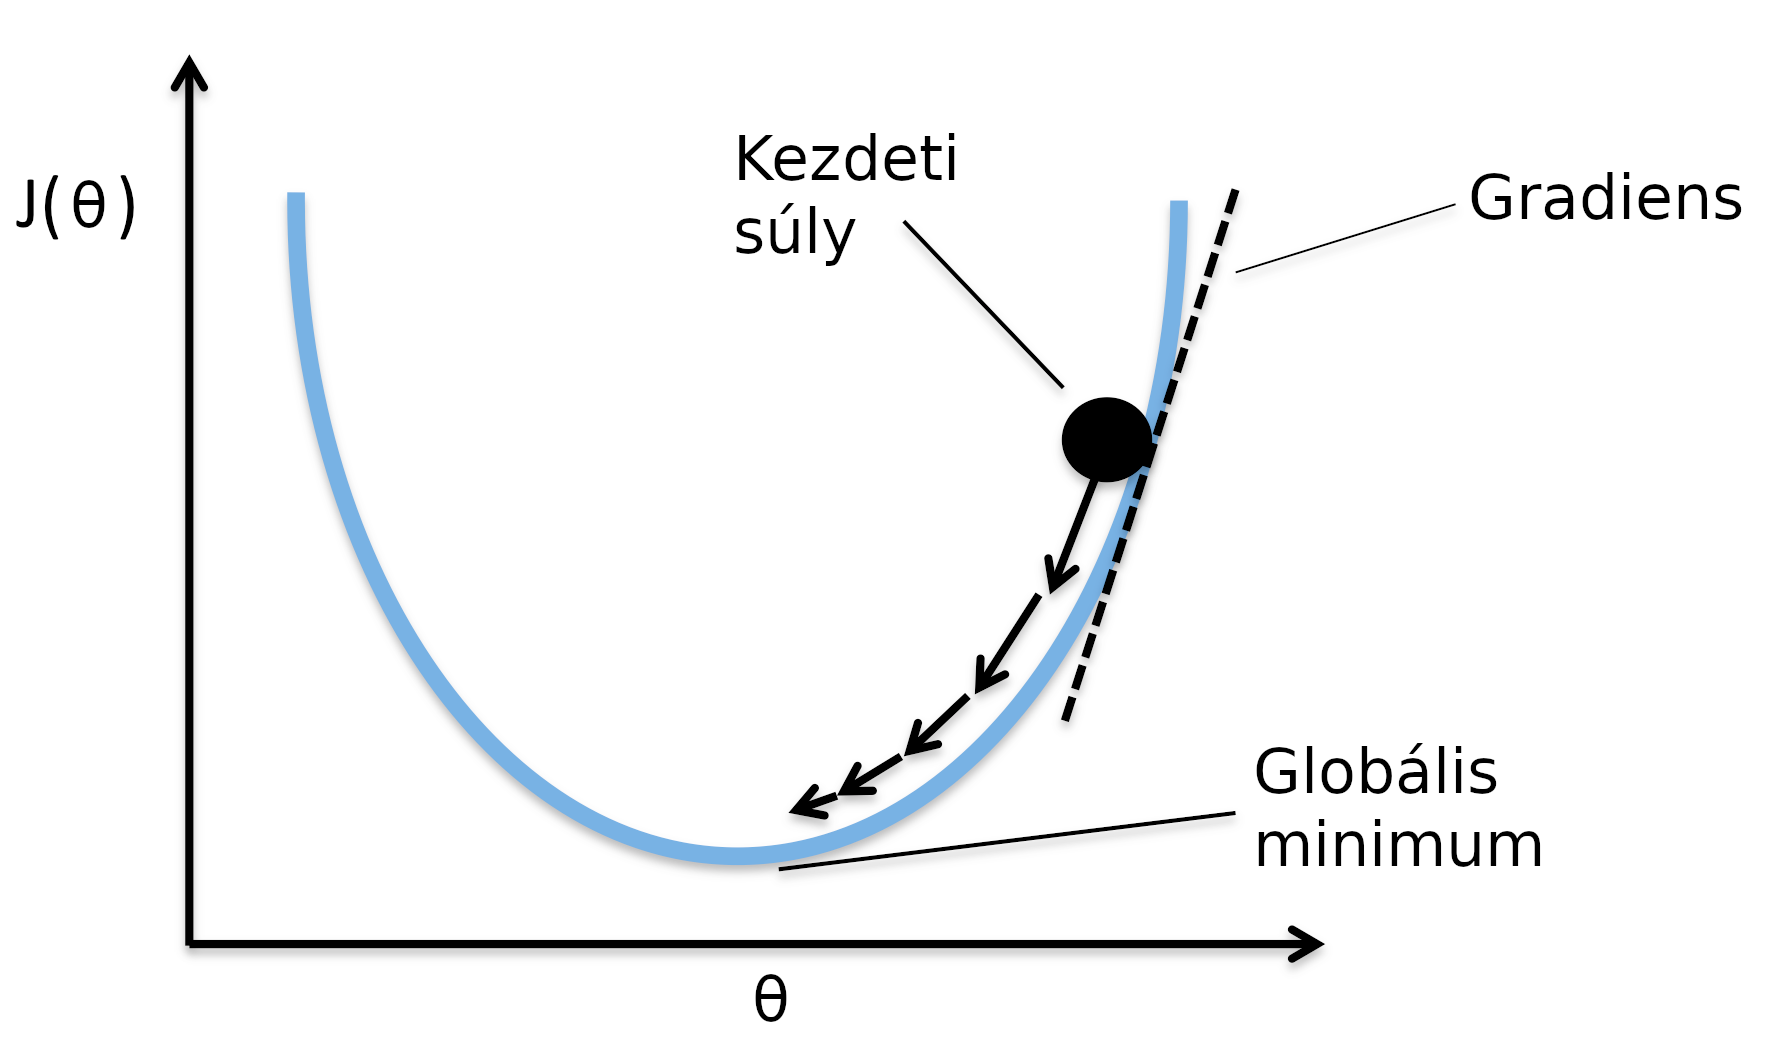
\includegraphics[width=7cm, height=7cm, keepaspectratio]{images/regresszio_19.png}
\end{center}
\end{column}
\end{columns}
\end{frame}

\begin{frame}{Gradiens ereszkedés optimális esetben}
\begin{columns}
\begin{column}{.5\textwidth}
\begin{center}
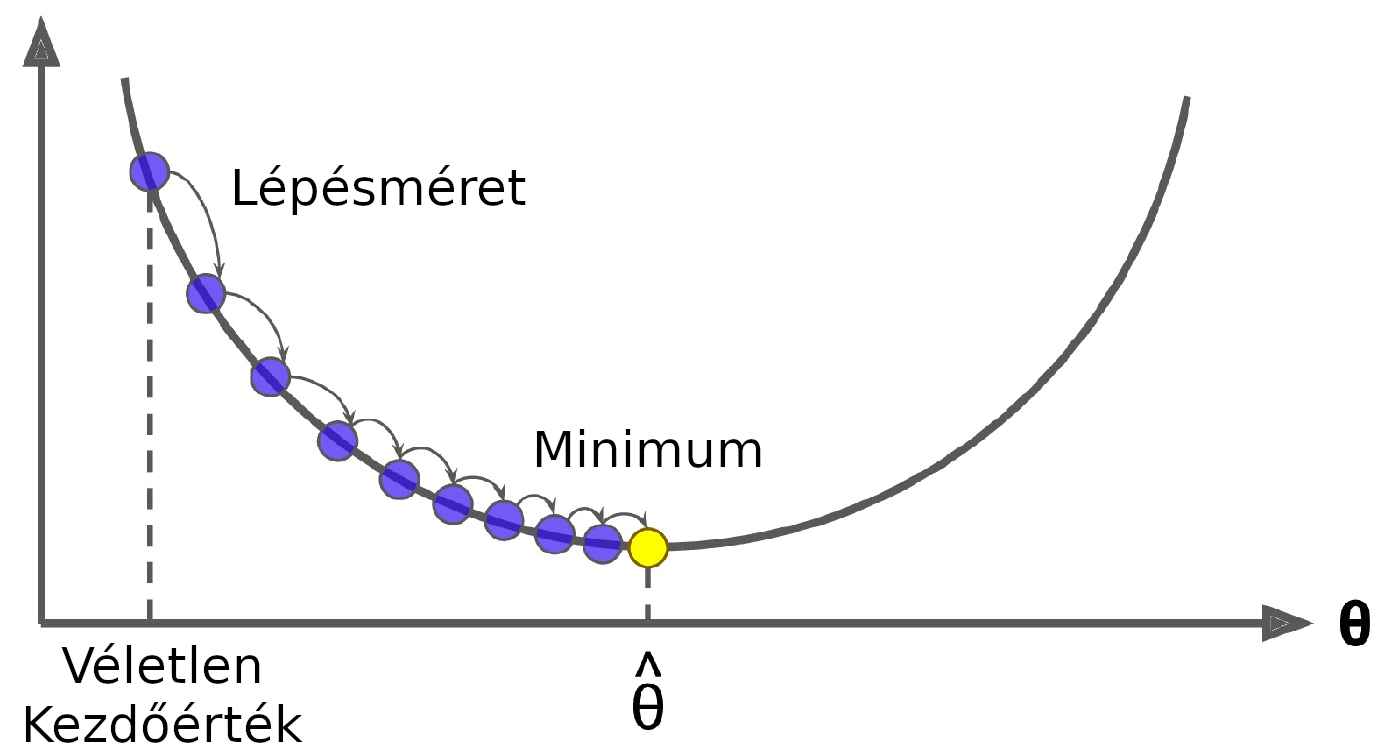
\includegraphics[width=7cm, height=7cm, keepaspectratio]{images/regresszio_20.png}
\end{center}
\end{column}
\begin{column}{.5\textwidth}
\begin{center}
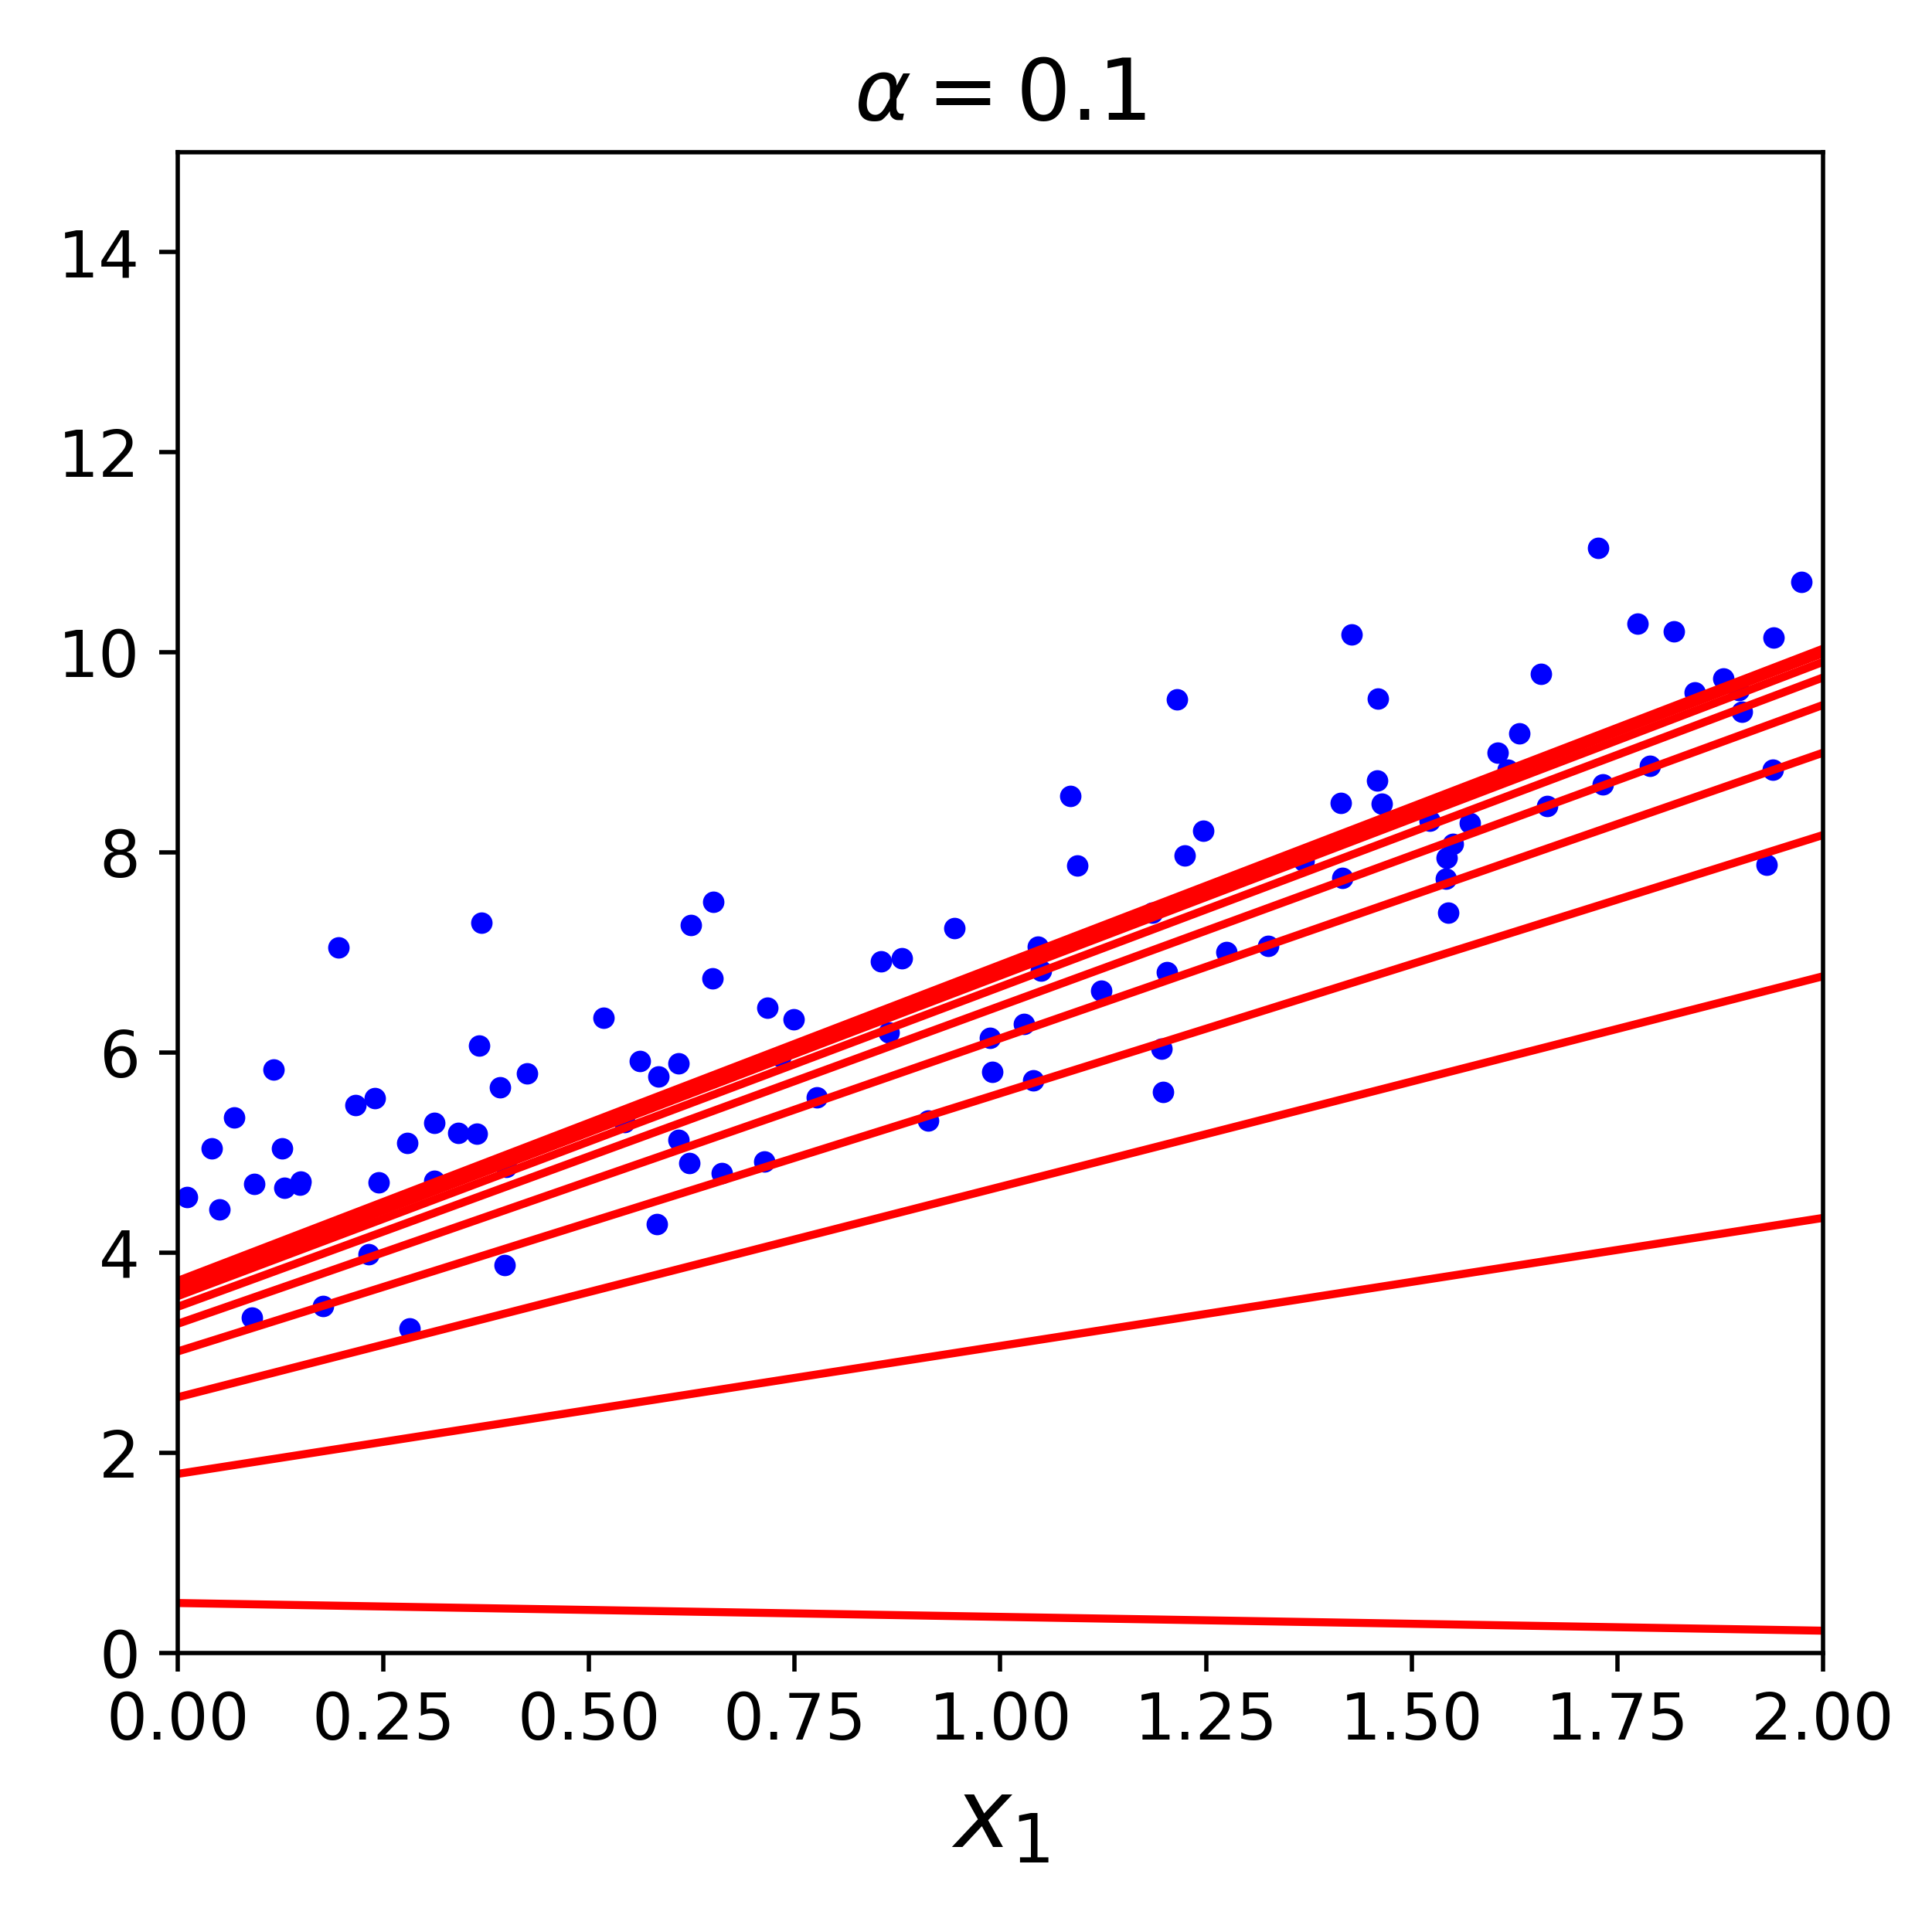
\includegraphics[width=7cm, height=7cm, keepaspectratio]{images/regresszio_25.png}
\end{center}
\end{column}
\end{columns}
\end{frame}

\begin{frame}{Túl alacsony tanulási sebesség}
\begin{columns}
\begin{column}{.5\textwidth}
Ha a tanulási sebesség túlságosan alacsony, az optimalizáció lehet sosem éri el a minimumot.
\begin{center}
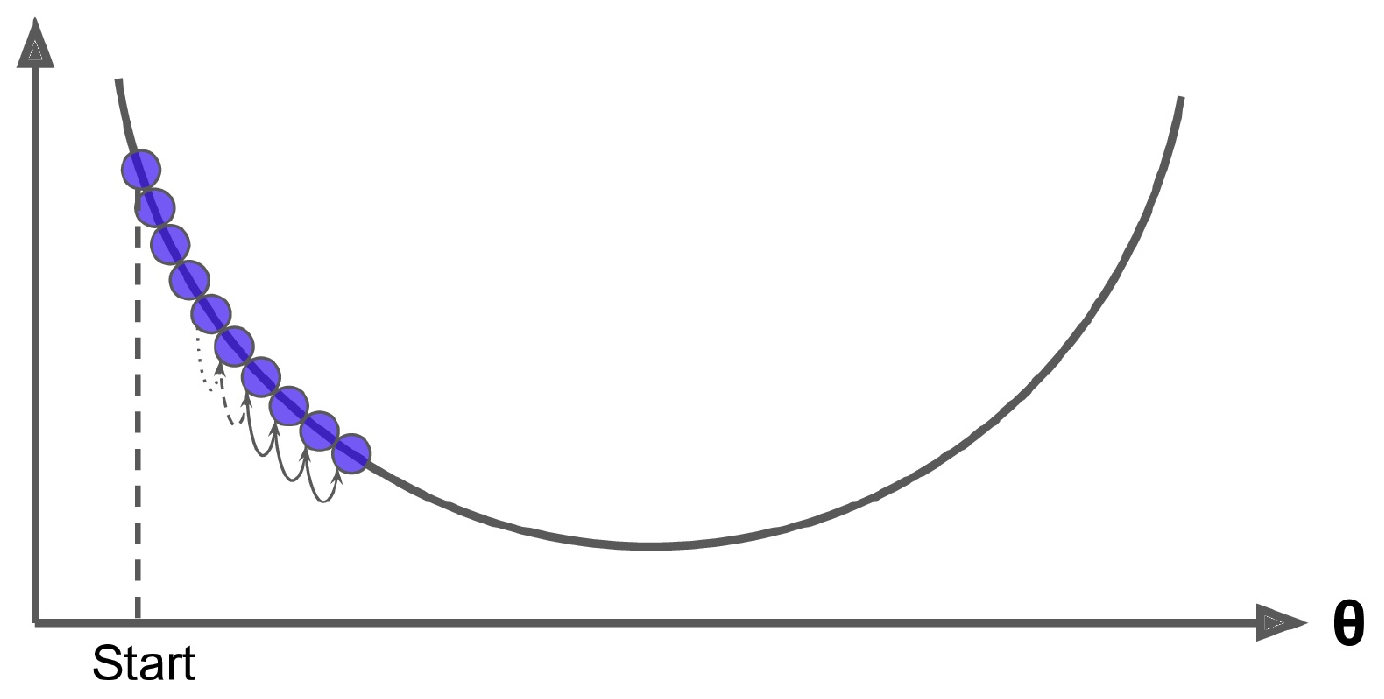
\includegraphics[width=7cm, height=7cm, keepaspectratio]{images/regresszio_21.png}
\end{center}
\end{column}
\begin{column}{.5\textwidth}
\begin{center}
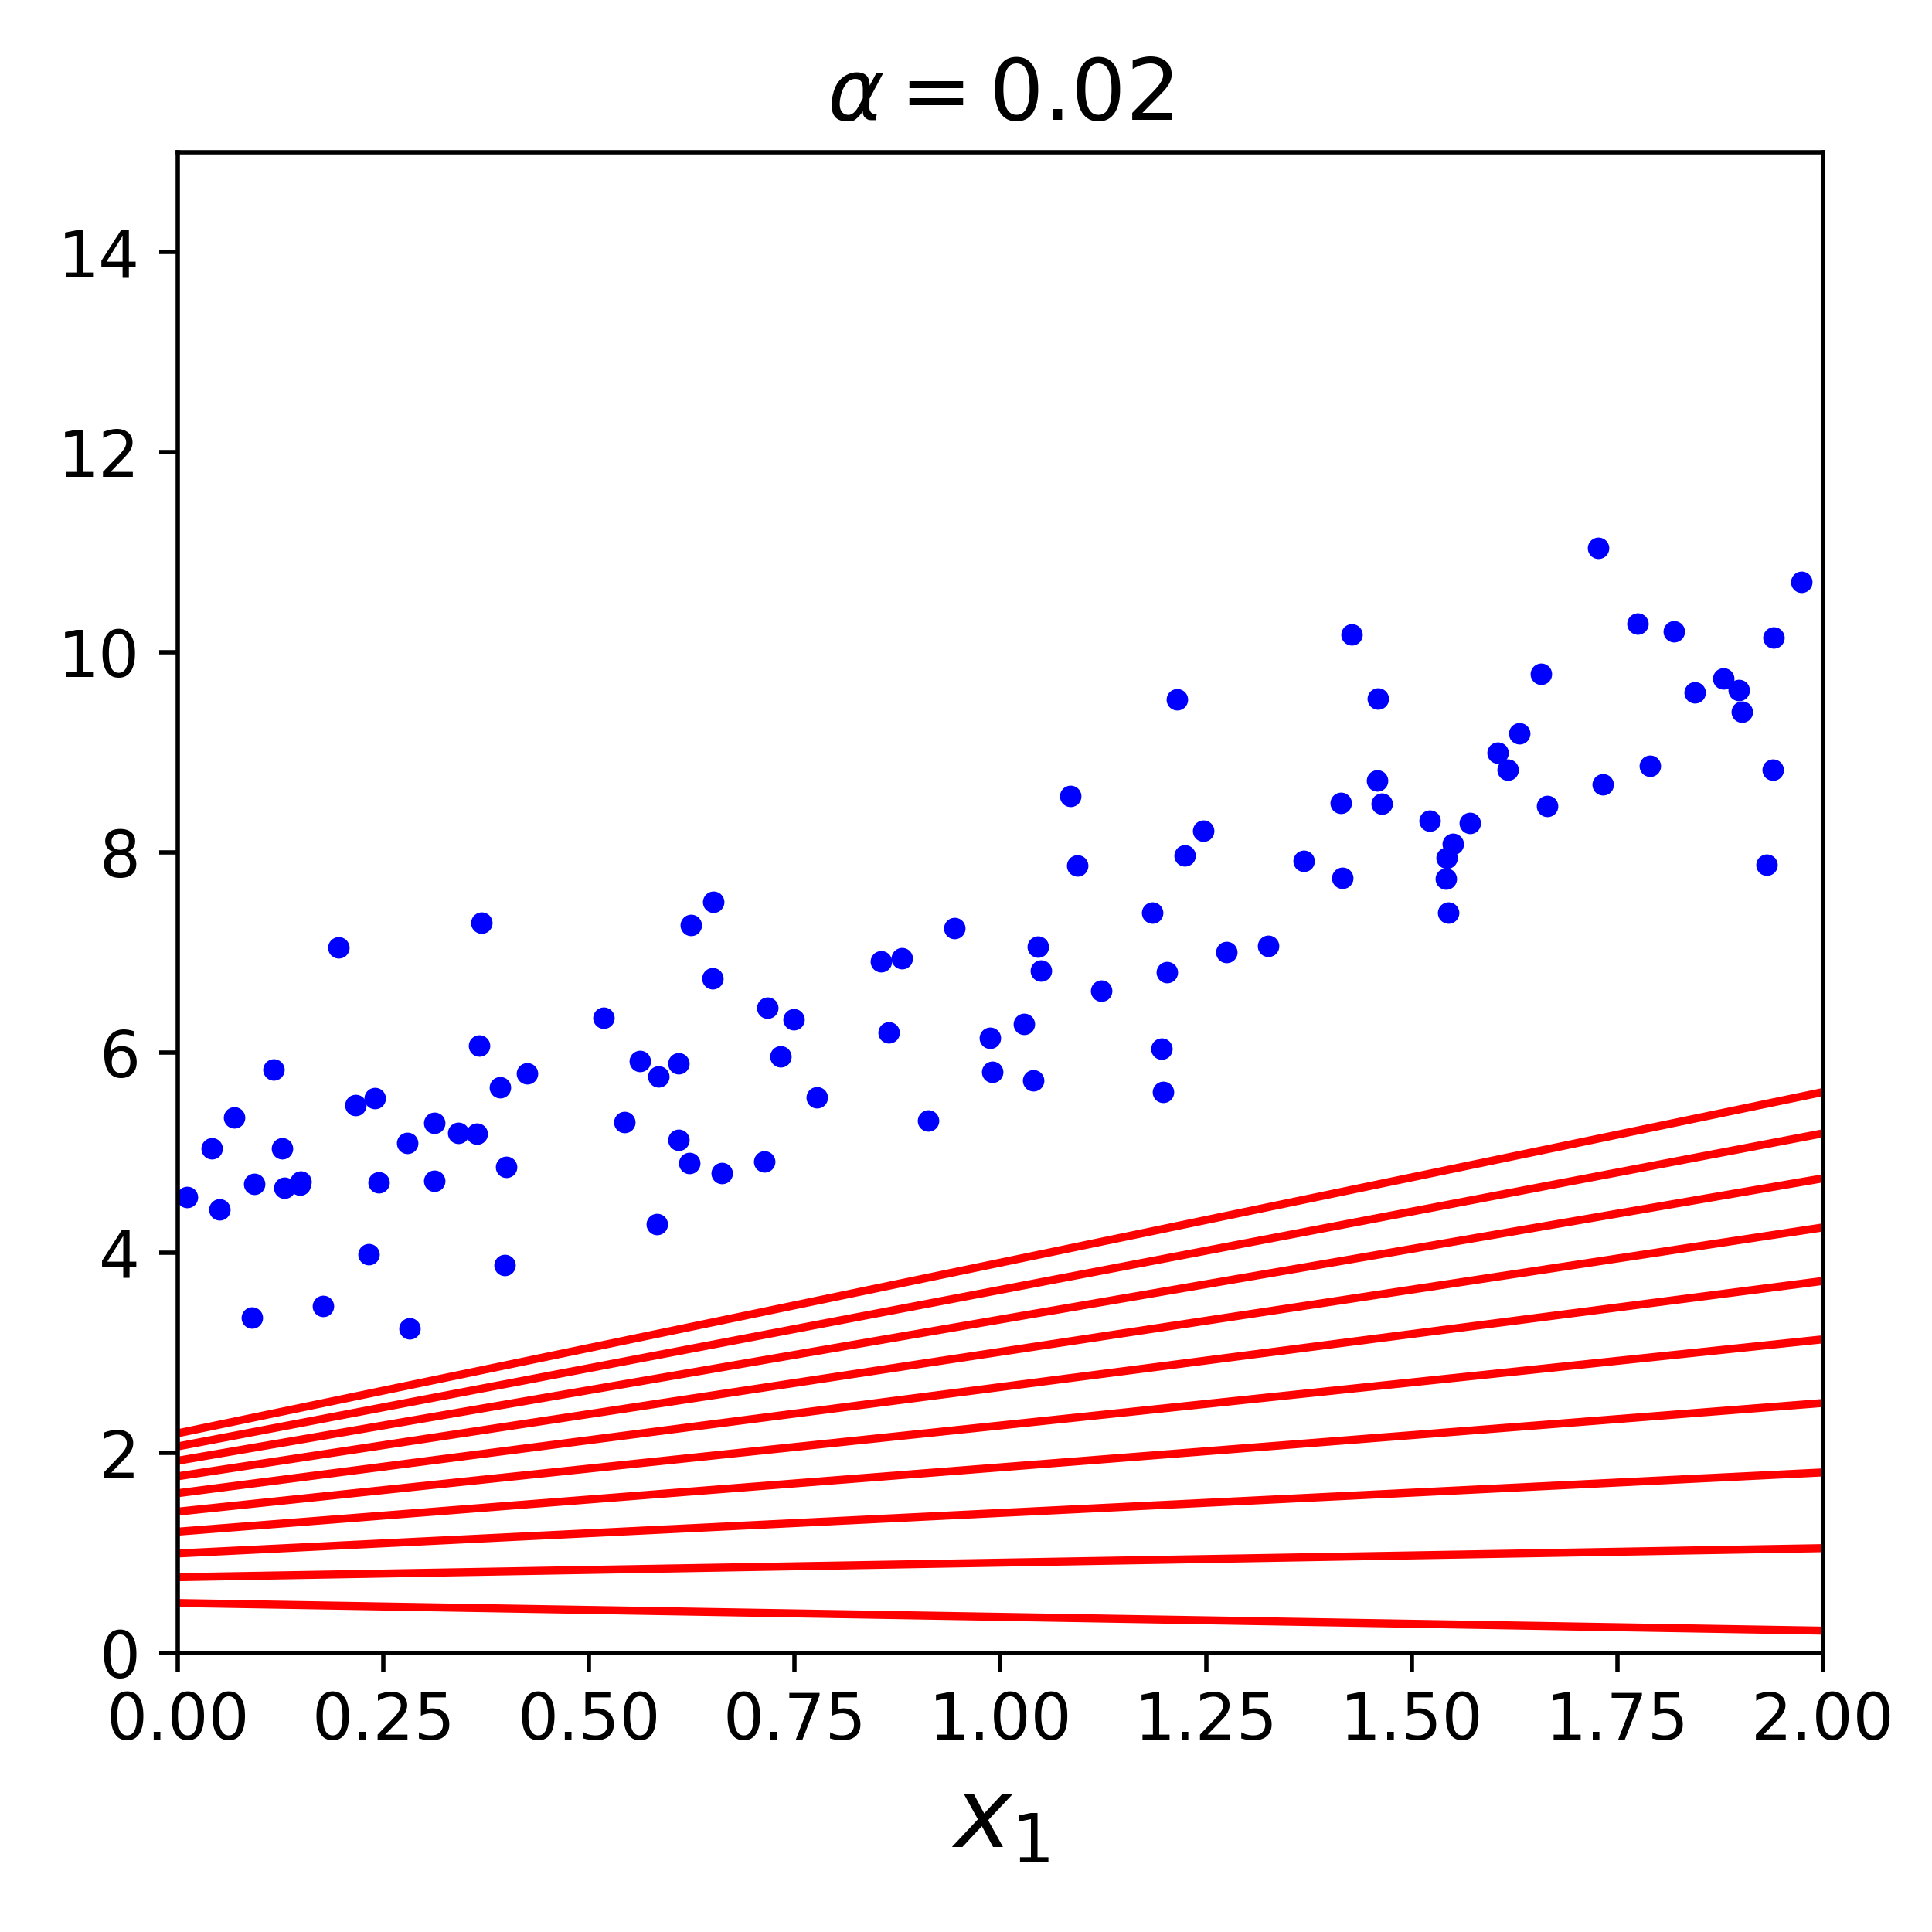
\includegraphics[width=7cm, height=7cm, keepaspectratio]{images/regresszio_24.png}
\end{center}
\end{column}
\end{columns}
\end{frame}

\begin{frame}{Túl magas tanulási sebesség}
\begin{columns}
\begin{column}{.5\textwidth}
Túlságosan magas tanulási sebesség esetén az algoritmus divergálhat vagy nagyon lassú lesz az optimalizáció folyamata. 
\begin{center}
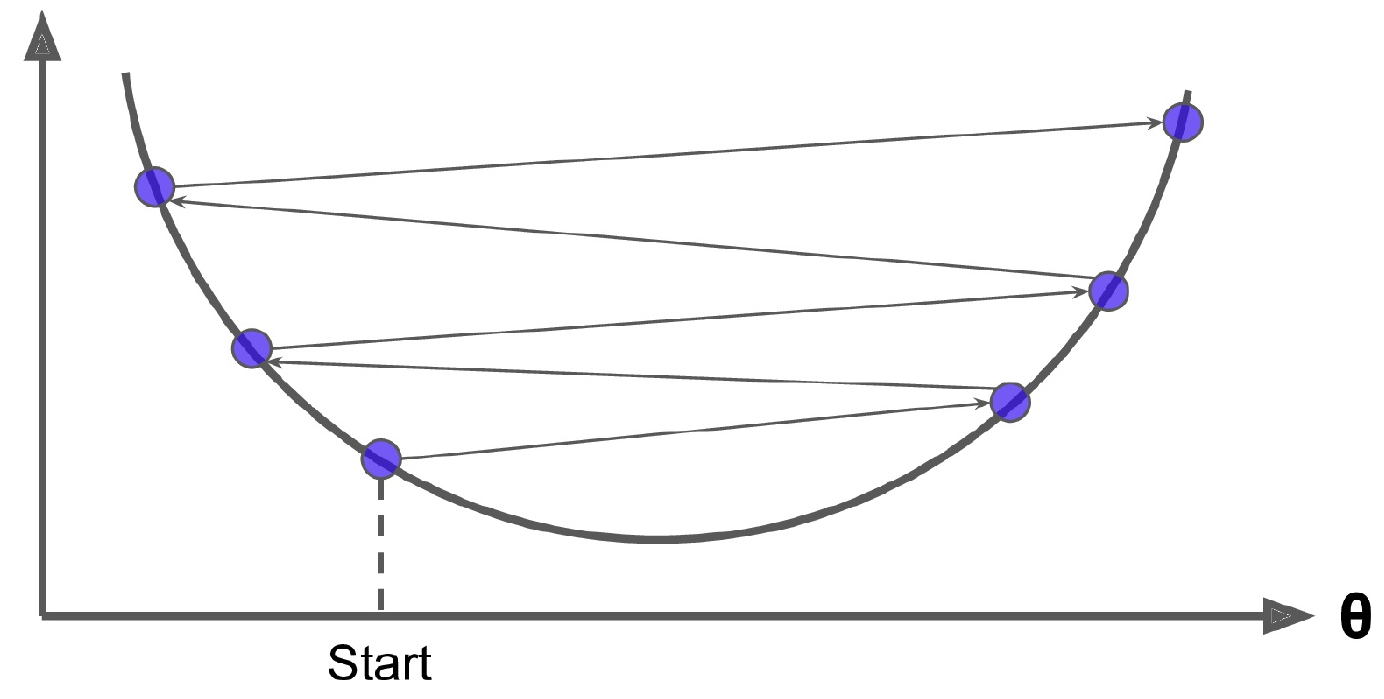
\includegraphics[width=7cm, height=7cm, keepaspectratio]{images/regresszio_22.png}
\end{center}
\end{column}
\begin{column}{.5\textwidth}
\begin{center}
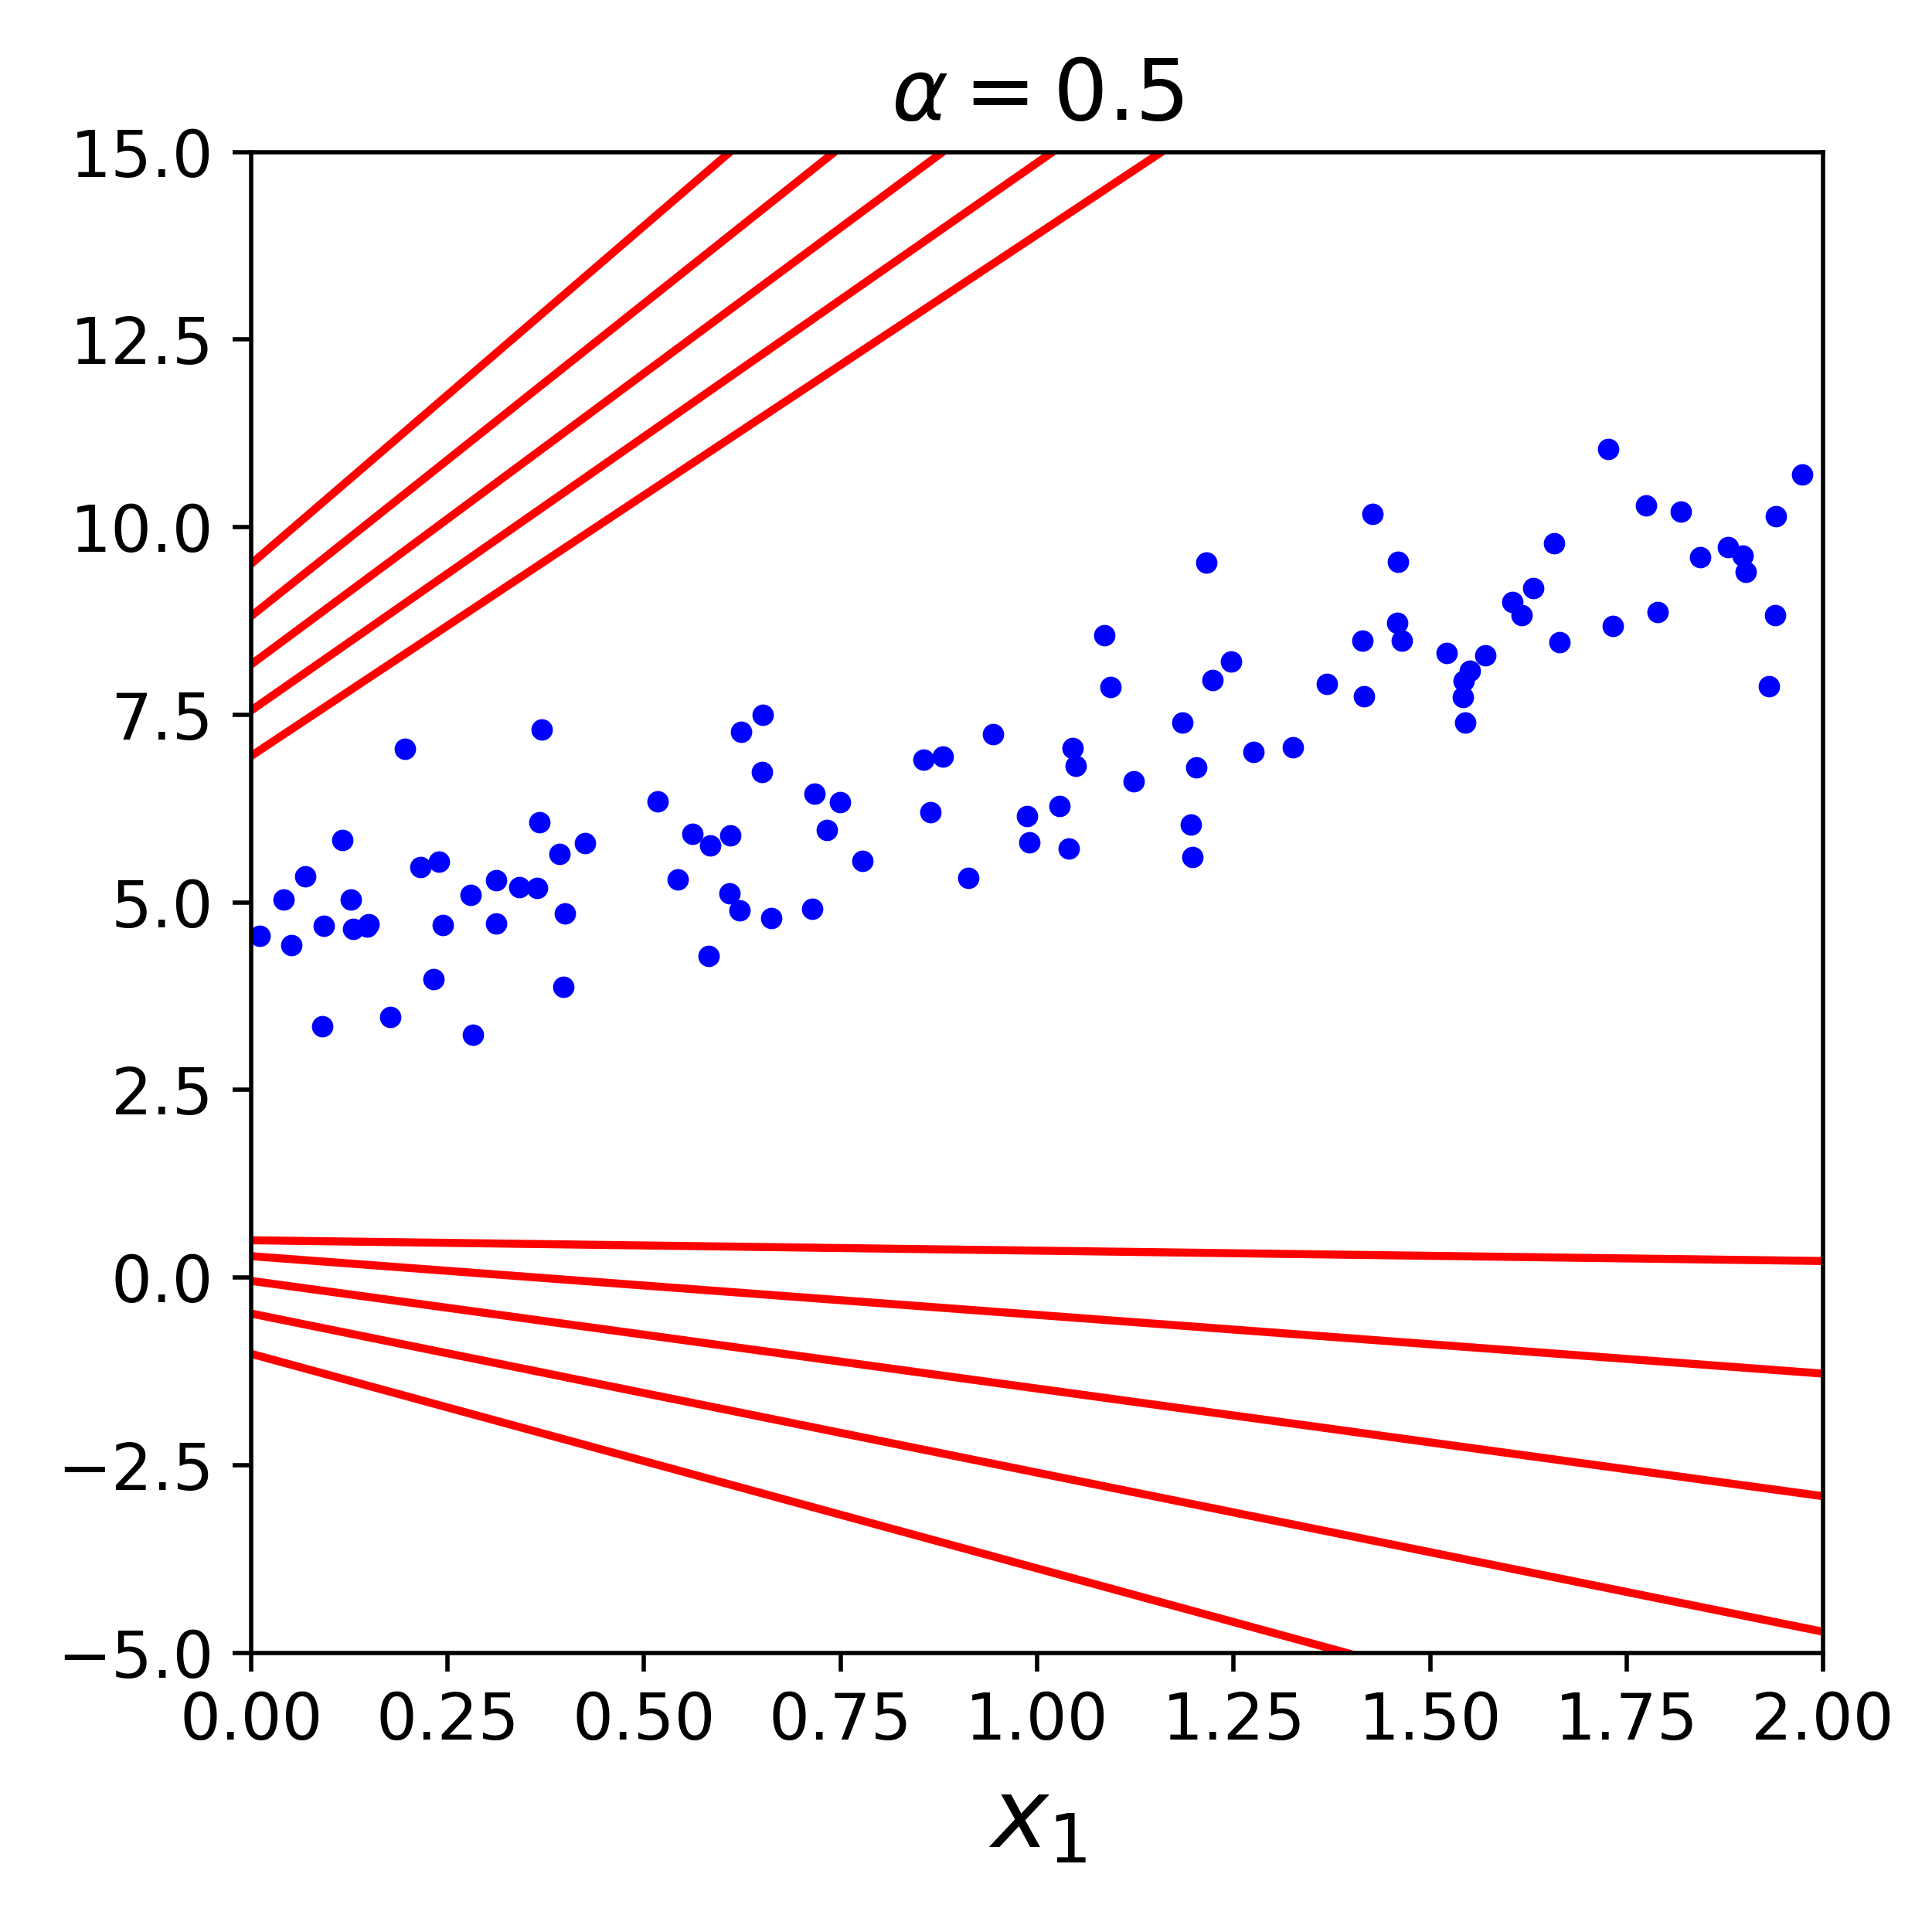
\includegraphics[width=7cm, height=7cm, keepaspectratio]{images/regresszio_26.png}
\end{center}
\end{column}
\end{columns}
\end{frame}

\begin{frame}{Egyéb problémák}
\begin{columns}
\begin{column}{.5\textwidth}
\begin{center}
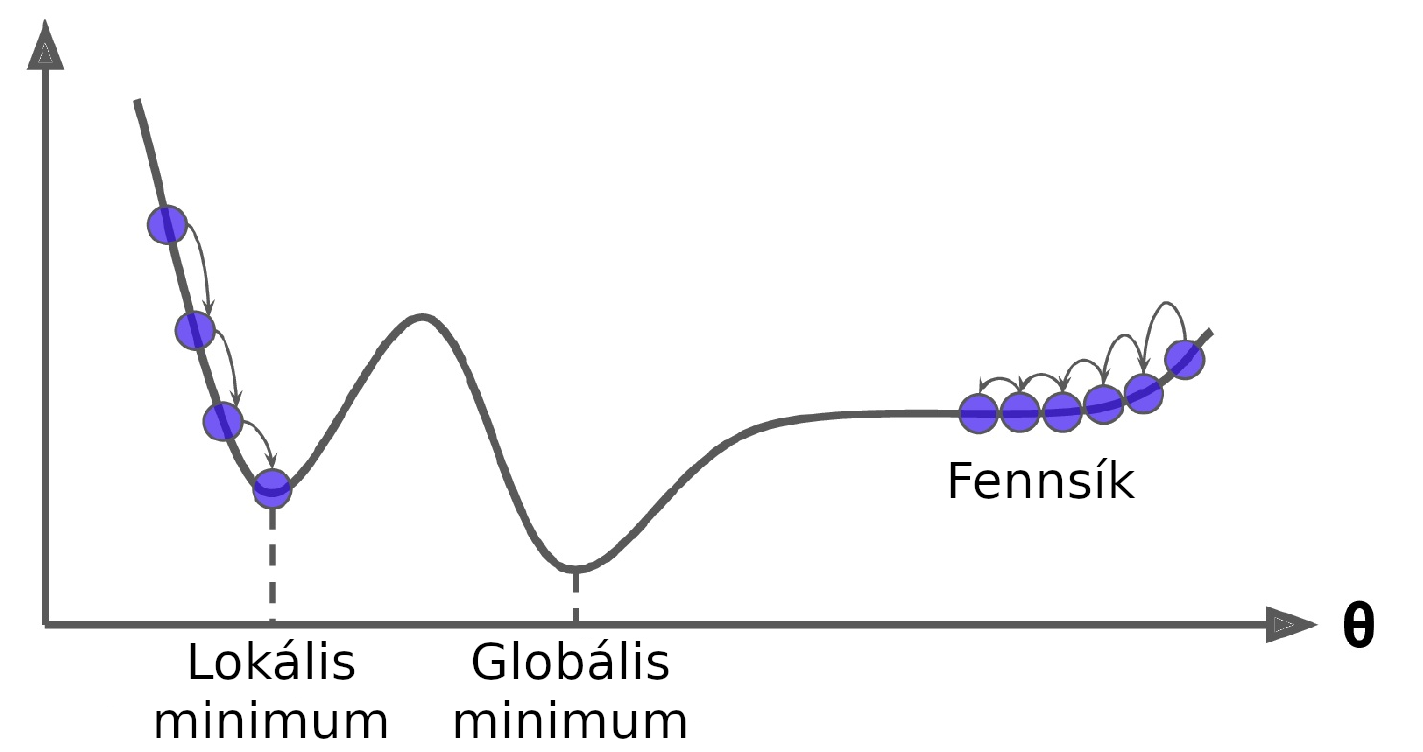
\includegraphics[width=7cm, height=7cm, keepaspectratio]{images/regresszio_23.png}
\end{center}
\end{column}
\begin{column}{.5\textwidth}
\begin{itemize}
	\item Az optimalizáció folyamata megakadhat egy lokális minimum helyen.
	\item Ha az algoritmus elér egy fennsíkot, az alacsony gradiens érték miatt instabillá válhat.
\end{itemize}
\end{column}
\end{columns}
\end{frame}

\end{document}




















